\documentclass[11pt,a4paper]{article} % ein Artikel in 11-Punkt Schrift
% wie man sich schon denkt leitet % einen Kommentar bis Zeilenende ein

\usepackage[german]{babel} % deutsch, deutsche Rechtschreibung
\usepackage[english]{}
\usepackage[utf8]{inputenc} % Unicode Text 
\usepackage[T1]{fontenc} % Umlaute und deutsches Trennen
\usepackage{mathptmx} % Times New Roman, gewohnter Font
\usepackage{courier} % Schreibmaschinenfont schicker
\usepackage[scaled=.95]{helvet} % was serifenloses wenn gebraucht
\usepackage{graphicx} % wir wollen Bilder einf��gen

\usepackage{listings} % Sch��ne Quellcode-Listings
\usepackage{color}

\definecolor{dkgreen}{rgb}{0,0.6,0}
\definecolor{gray}{rgb}{0.5,0.5,0.5}
\definecolor{mauve}{rgb}{0.58,0,0.82}

\lstset{frame=tb,
  language=Php,
  showstringspaces=false,
  columns=flexible,
  basicstyle={\small\ttfamily},
  numberstyle=\tiny\color{gray},
  keywordstyle=\color{blue},
  commentstyle=\color{dkgreen},
  stringstyle=\color{mauve},
  breaklines=true,
  breakatwhitespace=true,
  tabsize=3
}

% und eine eigene Umgebung f��r Listings
\usepackage{float}
\newfloat{listing}{htbp}{scl}[section]
\floatname{listing}{Listing}

% Auch wenn es anr��chig ist, man kann den Platz etwas mehr ausn��tzen
\usepackage[paper=a4paper,width=14cm,left=35mm,height=22cm]{geometry}
\usepackage{setspace}
\linespread{1.10} % nicht ganz anderthalbzeilig, nur ein bisschen mehr Platz
\setlength{\parskip}{0.5em} % kleiner Paragraphenabstand
\setlength{\parindent}{0em} % im Deutschen Einr��ckung nicht ��blich, leider

% Seitenmarkierungen 
\usepackage{fancyhdr} % Schickere Header und Footer
\pagestyle{fancy}
% font f��r Header/Footer
\newcommand{\phv}{\fontfamily{phv}\fontseries{m}\fontsize{9}{11}\selectfont}
\fancyhead[L]{\phv Praktikumsbericht} 
\fancyhead[R]{\phv \thepage}
\fancyfoot[L]{\phv Aoe GmbH}
\fancyfoot[C]{\ } % keine Seitenzahl unten
\fancyfoot[R]{\phv Michael Sandritter}

% Ein spezielles Paket zum Aufteilen des Literaturverzeichnisses
\usepackage{bibtopic}
\makeatletter
\def\@seccntformat#1{%
  \expandafter\ifx\csname c@#1\endcsname\c@section\else
  \csname the#1\endcsname\quad
  \fi}
\makeatother

\title{Praktikumsbericht}
\author{Michael Sandritter \\ AOE GmbH}

\date{\today}

\begin{document}
\maketitle % erzeugt den Titel mit Autor und Datum


\newpage % neue Seite, muss bei einem Artikel eigentlich nicht sein

\section{Praktikumsbetrieb} \label{sec:betrieb} 
% mit \label k��nnen wir die Einf��hrung referenzieren

Mein Praktikum habe ich bei der AOE GmbH in Wiesbaden absolviert. 
Die AOE GmbH hat seinen Hauptsitz in Wiesbaden und ist Dienstleister für Open
Source Enterprise Lösungen.
AOE wurde 1999 unter dem Firmennamen AOE media gegründet und arbeitete
anfänglich als TYPO3 Dienstleister.
Inzwischen umfassen die Serviceleistungen Open Source Web Portale, E-Commerce und mobile Anwendungen, 
die für globale agierende Unternehmen entwickelt werden. 
Das Kollegium umfasst 180 Entwickler und Consultants an 8 Standorten, davon 120 Mitarbeiter in der Zentrale in Wiesbaden. 
Die Unternehmenskultur setzt auf die Kernelemente: Open Source, objektorientierte Programmierung und Methoden 
wie Agile Software-Entwicklung und Test-Driven-Development. 

Dabei pflegt die AOE GmbH eine dezentrale Unternehmensstruktur. Jedem Kunden wird ein Team aus Entwicklern zur Seite gestellt. 
Das Team arbeitet von dort ab komplett selbstständig und setzt alle
Projektphasen in engem Kontakt mit dem Kunden um.

\section{Arbeitsumfeld} \label{sec:umfeld}

Während meines Praktikums arbeitete ich als PHP Backend-Entwickler im Congstar-Team.
Das Team bestand dabei aus 20 Entwicklern und acht Testern, die sich ihrerseits wiederum in 4 Sub-Teams aufteilen.
Die Frontend bzw. Backend-Kompetenzen waren dabei gleichmäßig auf die
verschiedenen Teams verteilt, so dass jedes Team, für sich, in der Lage war sowohl Backend- als auch
 Frontend-Tasks zu übernehmen.

Jedes Team arbeitet nach der agilen Softwareentwicklungsmethodik Scrum.
In täglichen Daily Meetings tauschen sich die Entwickler in ihren kleinen Teams über den aktuellen Entwicklungsstand aus, indem jeder Entwickler und Tester, dem Team erzählt, woran er gerade arbeitet und gegebenenfalls schildert welche Probleme bei der Umsetzung existieren.
Zusätzlich finden zwei mal wöchentlich “Weekly“ Meetings statt, bei denen alle Entwickler und Tester zu einem übergreifenden Update des Entwicklungsstand zusammenkommen.
In der großen Runde werden Themen besprochen, die das komplette Team betreffen.
Dazu gehört zum Beispiel, das Einführen und Verwenden neuer Technologien, das Entwickeln oder ändern der Software Architektur und generelle organisatorische Themen.

Während der täglichen Arbeit wird jedes Team von einem IT Analysten (ITA) von Congstar betreut. Dieser hat die Funktion des Scrummasters inne und moderiert beispielsweise die Dailys und Sprint Retrospektiven (dazu später mehr). Außerdem ist er die Schnittstelle zwischen dem Kunden und dem Team. Er ist Ansprechpartner für das Team bei Problemen oder fehlenden Informationen. Er kennt die Abläufe bei Congstar und weiß welcher Ansprechpartner für welches Anliegen der richtige ist.

Der zeitliche Rahmen gibt vor, dass dem Kunden alle zwei Monate ein neues Softwarepaket mit neuen Features ausgeliefert wird.
Innerhalb dieser Zeit absolviert, jedes Team drei Sprints. Die ersten beiden Sprints sind Feature Sprints,
die jeweils 3 Wochen Arbeitszeit umfassen. In diesen beiden Sprints werden neue Stories umgesetzt,
die davor von den Product Ownern (PO) priorisiert worden sind. Das Team
entscheidet jedoch für jeden Sprint neu, wie viele Stories realistisch umsetzbar sind und arbeitet zu jeder Story kleinere Tasks aus,
die von den Entwicklern geclaimed (Ein Entwicker / Tester “nimmt“ sich eine offene Aufgabe und bearbeite diese) und umgesetzt werden. Der letzte Sprint innerhalb der zwei Monate ist ein Release Sprint.
Dieser erstreckt sich über die beiden verbleibenden Wochen.
Zu dieser Zeit finden Verbundtests statt, bei denen die neu entwickelten Features im Zusammenspiel mit der AAX$^{2}$ getestet werden.


\par
\begingroup
\leftskip=1cm % ggf. verstellen
\noindent Die AAX$^{2}$ ist eine Software aus dem Hause Compax (Compax Software Development GmbH ansässig in Wien, Österreich). Diese ist das Workflow-Management-System von Congstar und beinhaltet unteranderem den congstar-spezifischen Produktkatalog.
Darin werden alle Congstar Produkte abgebildet, wie zum Beispiel die Post- und
Prepaidtarife, mit den dazugehörigen Buchungsoptionen oder die von Congstar angebotenen Endgeräte mit ihren Produktdetails  \& ihrer Verfügbarkeit.
Die AAX$^{2}$ bietet zur Kommunikation mit Externen Anwendungen, Soap-Schnittstellen an. Über diese werden z.B.: die Produktdaten durch das von AOE System abgerufen.\cite{cx}
\par
\endgroup

Im laufe des Release Sprints, besteht für die Entwickler ein Feature-Entwicklungs-Stop, damit das neue Softwarepaket im Verbundtest getestet werden kann.
Anstatt an neuen Features zu arbeiten, wird die Zeit zum Beispiel zum Refactorn der Software, zum Updaten von Frameworks oder anderer Software genutzt. Alternativ wird auch neue Software oder Techniken ausprobiert und getestet oder vorhandene getestet und aufgeräumt.
Somit alles, was während der beiden Featuresprints liegen geblieben ist oder für was keine Zeit war, wird erledigt. Falls im Verbundtest Fehler auftreten, werden diese bewertet und falls kritisch behoben.

Am Ende jedes Sprints findet zusammen mit den Stakeholdern (Congstar PO's und ITA's) der Sprintwechsel statt, bei dem das Entwickler-Team die Ergebnisse des aktuell endenden Sprints präsentieren und den nächsten Sprint vorbereitet.
Dafür fahren die Entwickler-Teams nach jedem Feature-Sprint nach Köln zu Congstar und nach Ende des Release-Sprints treffen kommen die PO's und ITA's nach Wiesbaden und führen den Sprintwechsel bei AOE durch.
Hauptsächlich geht es um die Präsentation der Stories, die innerhalb des letzten Sprints erfolgreich umgesetzt werden konnten.
Das Entwickler-Team führt in diesem Zug auch eine Retrospektive des vergangenen Sprints durch und berichtet, was während des Sprints gut gelaufen ist, welche technischen Probleme und Hindernisse sich ergeben haben und wie diese Probleme gelöst wurden.
Die Stakeholder haben in diesem Zuge die Möglichkeit offene Fragen mit den Entwicklern direkt zu klären. Alle Beteiligten erhalten somit einen Überblick über den aktuellen Stand des Projekts.
Das Review dient als Grundlage für das darauf folgende Sprint Planning, als die Planung was im nächsten Sprint bearbeitet wird.
Grundlage des Plannings ist das Produkt-Backlog, dort werden durch die PO's Stories gesammelt, welche künftig umgesetzt werden sollen.
Diese Stories kommen durch neue Features aber auch Bugs in das Backlog und werden dann von den PO's  priorisiert.

Während des Sprint Plannings werden im ersten Teil die Stories im Backlog gegroomt, also abgeschätzt wie aufwendig die Stories sind.
Als Ergebnis des Groomings werden der Story Punkte zugewiesen, diese dienen dem Vergleich der Stories untereinander und der Abschätzung des gesamten Sprintumfangs. Eigentlich vergleicht man Punkte nicht mit einer Zeit Einheit, jedoch erhält jedes Teammitglied im Laufe des Projekts ein Gefühl dafür wie Aufwendig bestimmte Aufgaben sind und wie viel das Team im Laufe einer Arbeitswoche umsetzen kann. Anfangs waren Beispielsweise meine geschätzten Punkte sehr stark abweichend von denen meiner Teammitglieder, mit der Zeit habe ich aber relativ schnell ein Gefühl dafür bekommen.
Im zweiten Teil des Plannings werden die nun gegroomten Stories im Backlog durch die PO's nochmals mit den neuen Informationen bezüglich des Aufwands priorisiert und dann wird durch das Entwicklerteam festgelegt wird wie viele der besprochenen Stories umgesetzt werden können. Das hier gesetzte Sprintziel sollte möglich sein und die Entwickler versichern, mit ihrer Aussage, dass es auch geschafft wird.

Falls Stories schneller umgesetzt werden als geplant, kann immer eine Story aus dem Backlog nachgezogen werden, jedoch sollte dies das Sprintziel nicht beeinflussen. Falls ungeplante Ereignisse oder Abhängigkeiten eintreten, welche eine Story verzögern, kann diese überkippen in den nächsten Sprint, jedoch sollte dies möglichst vermieden werden.

Nachdem die Stories für den nächsten Sprint festgelegt sind, definieren die Entwickler für jede Story kleinere Aufgaben (Tasks) und schätzen diese in Minuten, Stunden und Tagen ab. Dabei ist es wichtig, die Aufgaben so klein wie Möglich und so groß wie nötig zu wählen.

In unserem Fall werden Backlog, Stories und Tasks im Projekt-
Management-Tool Jira verwaltet.

Im Laufe des Sprints werden die einzelnen Tasks von den Entwicklern abgearbeitet.
Zum beginn einer Aufgabe vermerkt der Entwickler im Jira, dass dieser nun daran arbeitet, indem er sich den Task claimed, also diesen auf “in Arbeit“ zieht und Jira dann automatisch den Benutzer an den Taks hängt.
Während der Arbeit wird an dem Tasks vermerkt, wie viel Zeit für den Task verbraucht wurde (geburned). Aus der
geschätzten und der letztendlich benötigten Zeit lässt sich ein Burndown-Chart ermitteln, das den aktuellen Fortschritt des Sprints widerspiegelt.

Sind alle Tasks einer Story umgesetzt steht die Abnahme dieser Story an. Diese erfolgt durch einen Entwickler der an der Umsetzung der Story beteiligt war und durch den Product Owner (PO).
Der Entwickler präsentiert dem PO die Features, die durch die Story umgesetzt werden sollten.
Erfüllt das Umgesetzte alle Akzeptanz-Kriterien, die für die Story definiert wurden, kann die Story durch den PO abgenommen werden und ist fertig.

\section{Projektbeschreibung} \label{sec:projekt}

Mein Team ist zuständig für die Congstar GmbH.

Congstar ist eine Tochterfirma der Deutschen Telekom AG und deutschlandweiter Anbieter für Mobilfunk- und DSL-Produkte.
2008 hat Congstar ein ambitioniertes Ziel: Die komplette IT von congstar sollte innerhalb eines Jahres komplett ersetzt werden.

AOE hat dabei für Congstar ein komplettes Telco E-Commerce Framework auf Basis des Open Source Content Management Systems (CMS) TYPO3 entwickelt und betreut es seit dem mit aktuell 3 Teams und somit ca. 15 Mitarbeitern allein für den Webbereich.

Congstar vermarktet all seine Produkte vorrangig über das Internet, somit ist das Web nahezu der Kern von Congstar. AOE übernimmt dabei die gesamte Web-Entwicklung bestehend aus: Content Management System, Produktkonfiguration und Bestellprozessen, Kampagnen-Management-System, Kundenservice, Vertriebspartnerportal und White Label-Vertrieb.

\begin{center}
\textbf{Webseiten und Portale}
\end{center}

\begin{figure}[H]
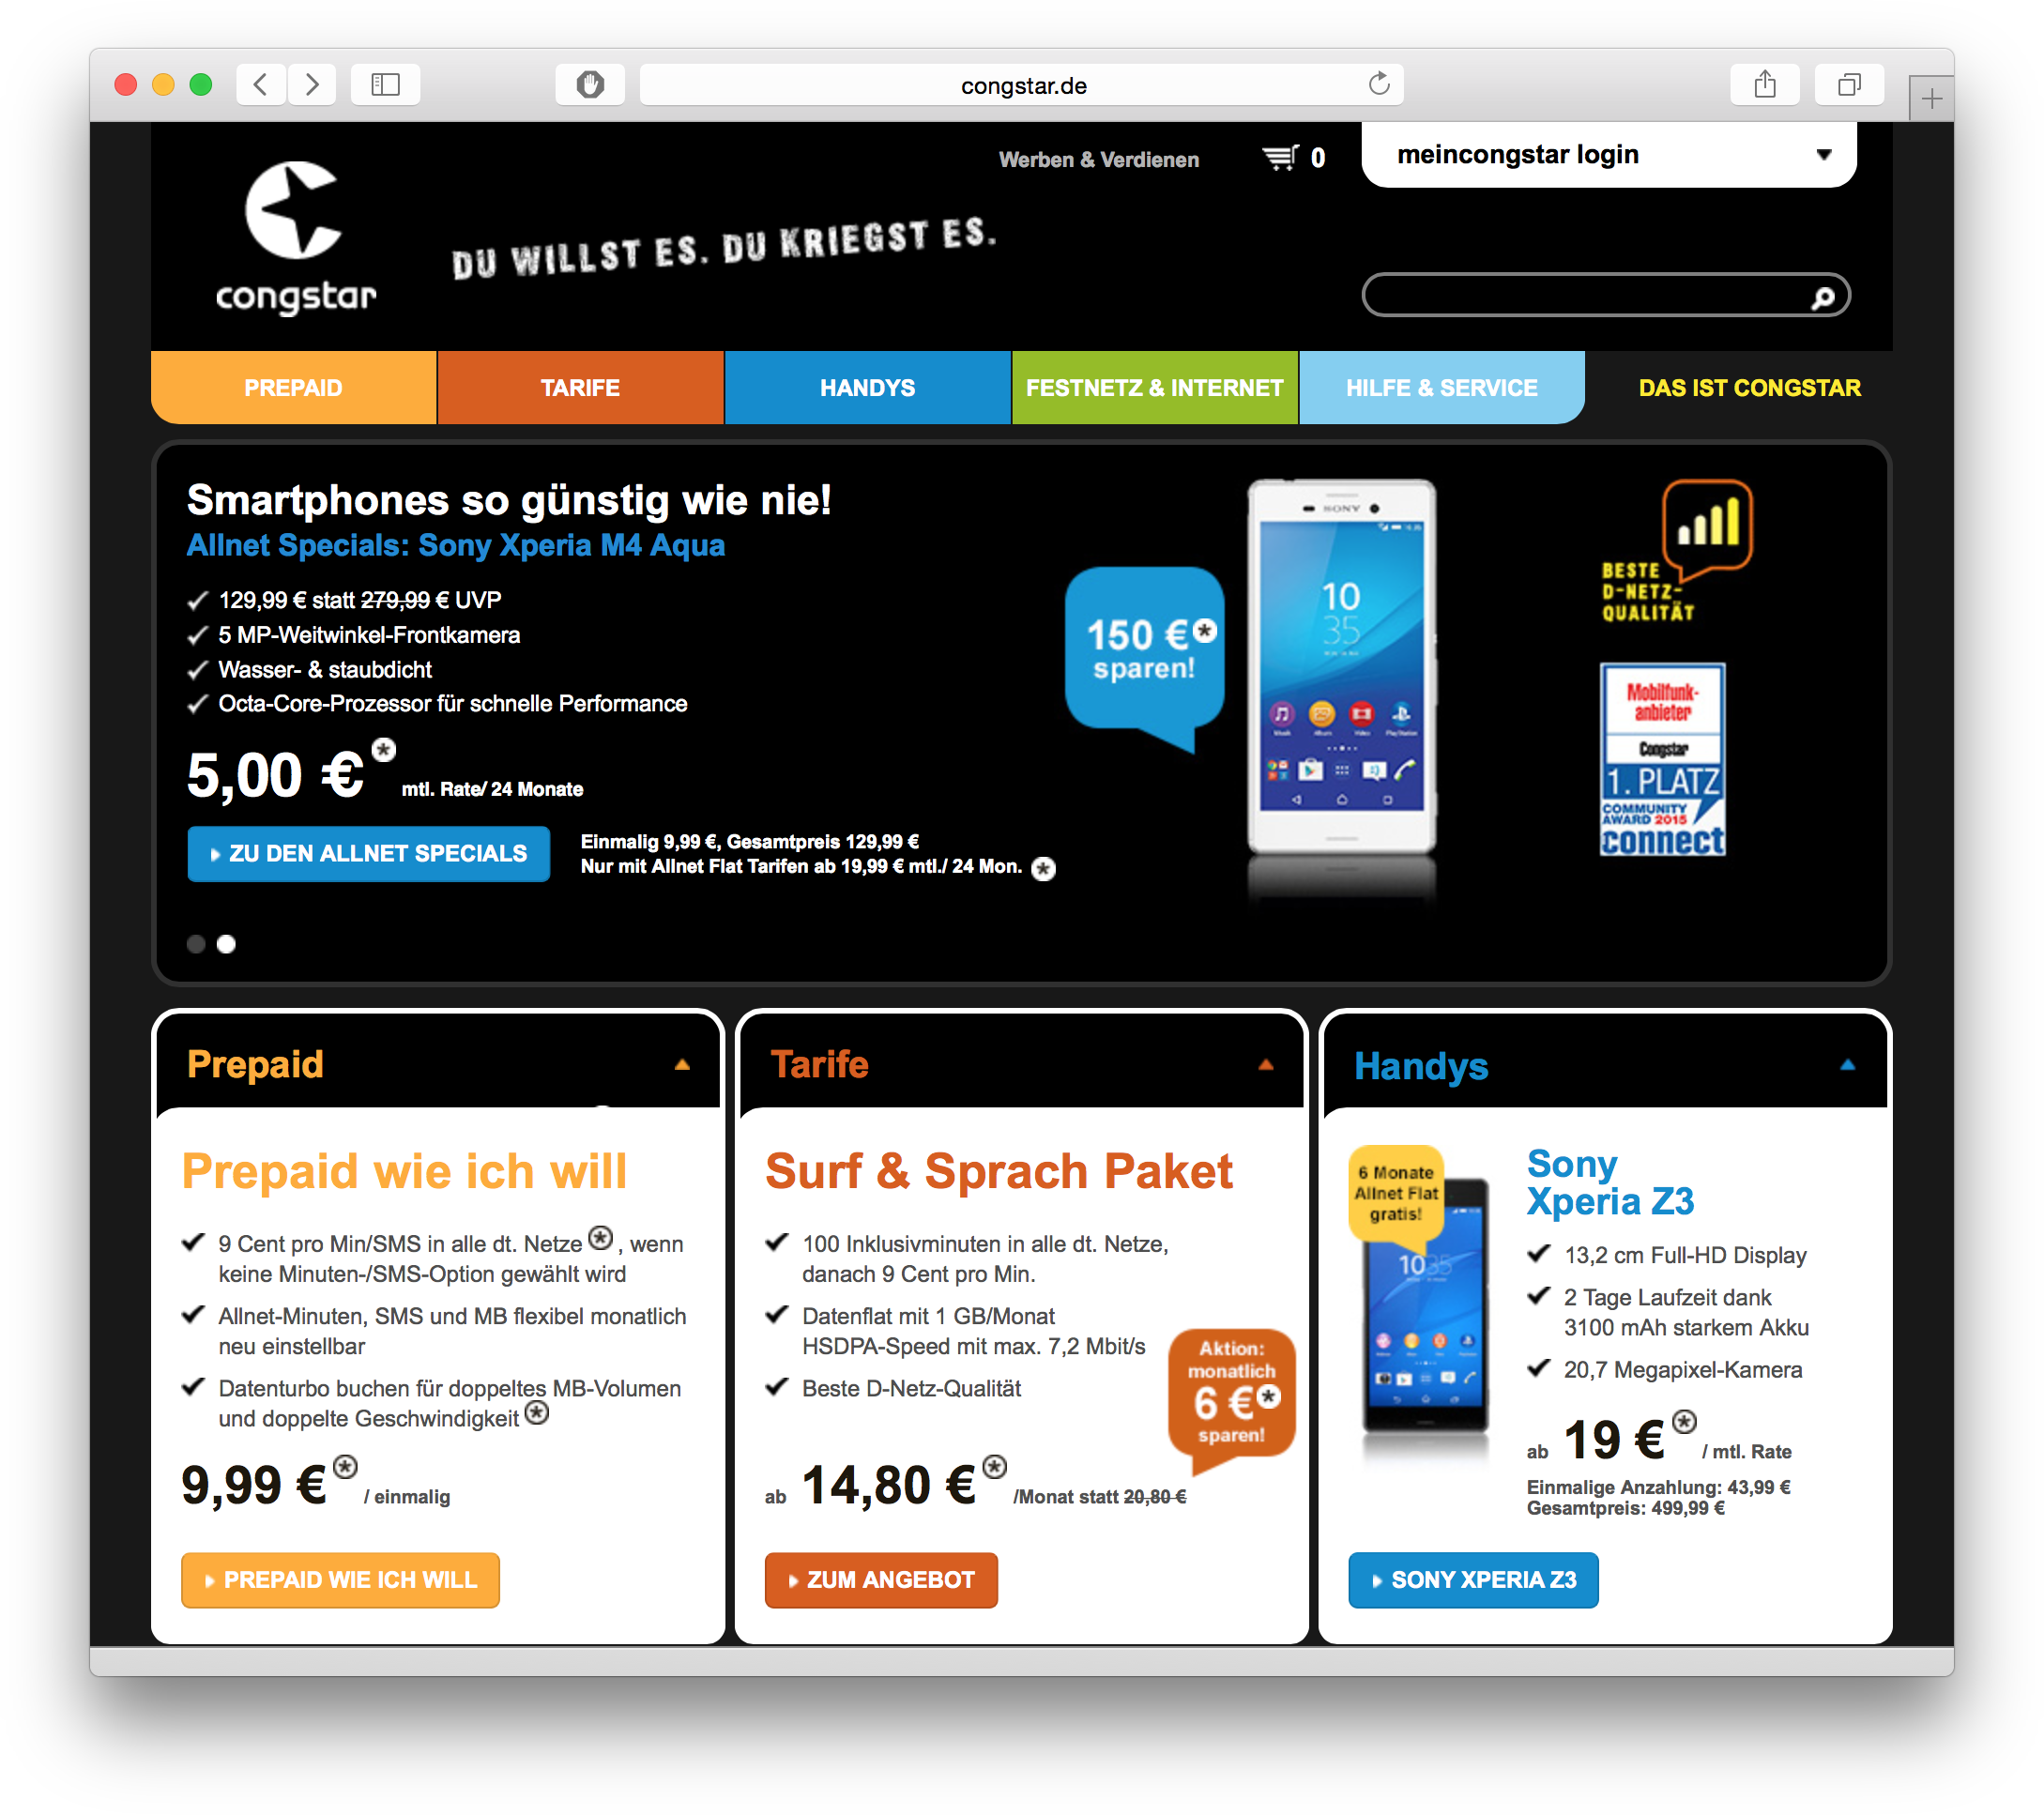
\includegraphics[width=0.7\textwidth]{images/Sites/Congstar_Main.png}
\centering
\caption{Die Congstar Hauptwebseite \cite{cmain}}
\end{figure}

\begin{figure}[H]

\includegraphics[width=0.7\textwidth]{images/Sites/Congstar_Mobil_CSC.png}
\centering
\caption{Das Congstar Mobil Kundenportal (CSC) \cite{ccsc}}
\end{figure}

\begin{figure}[H]
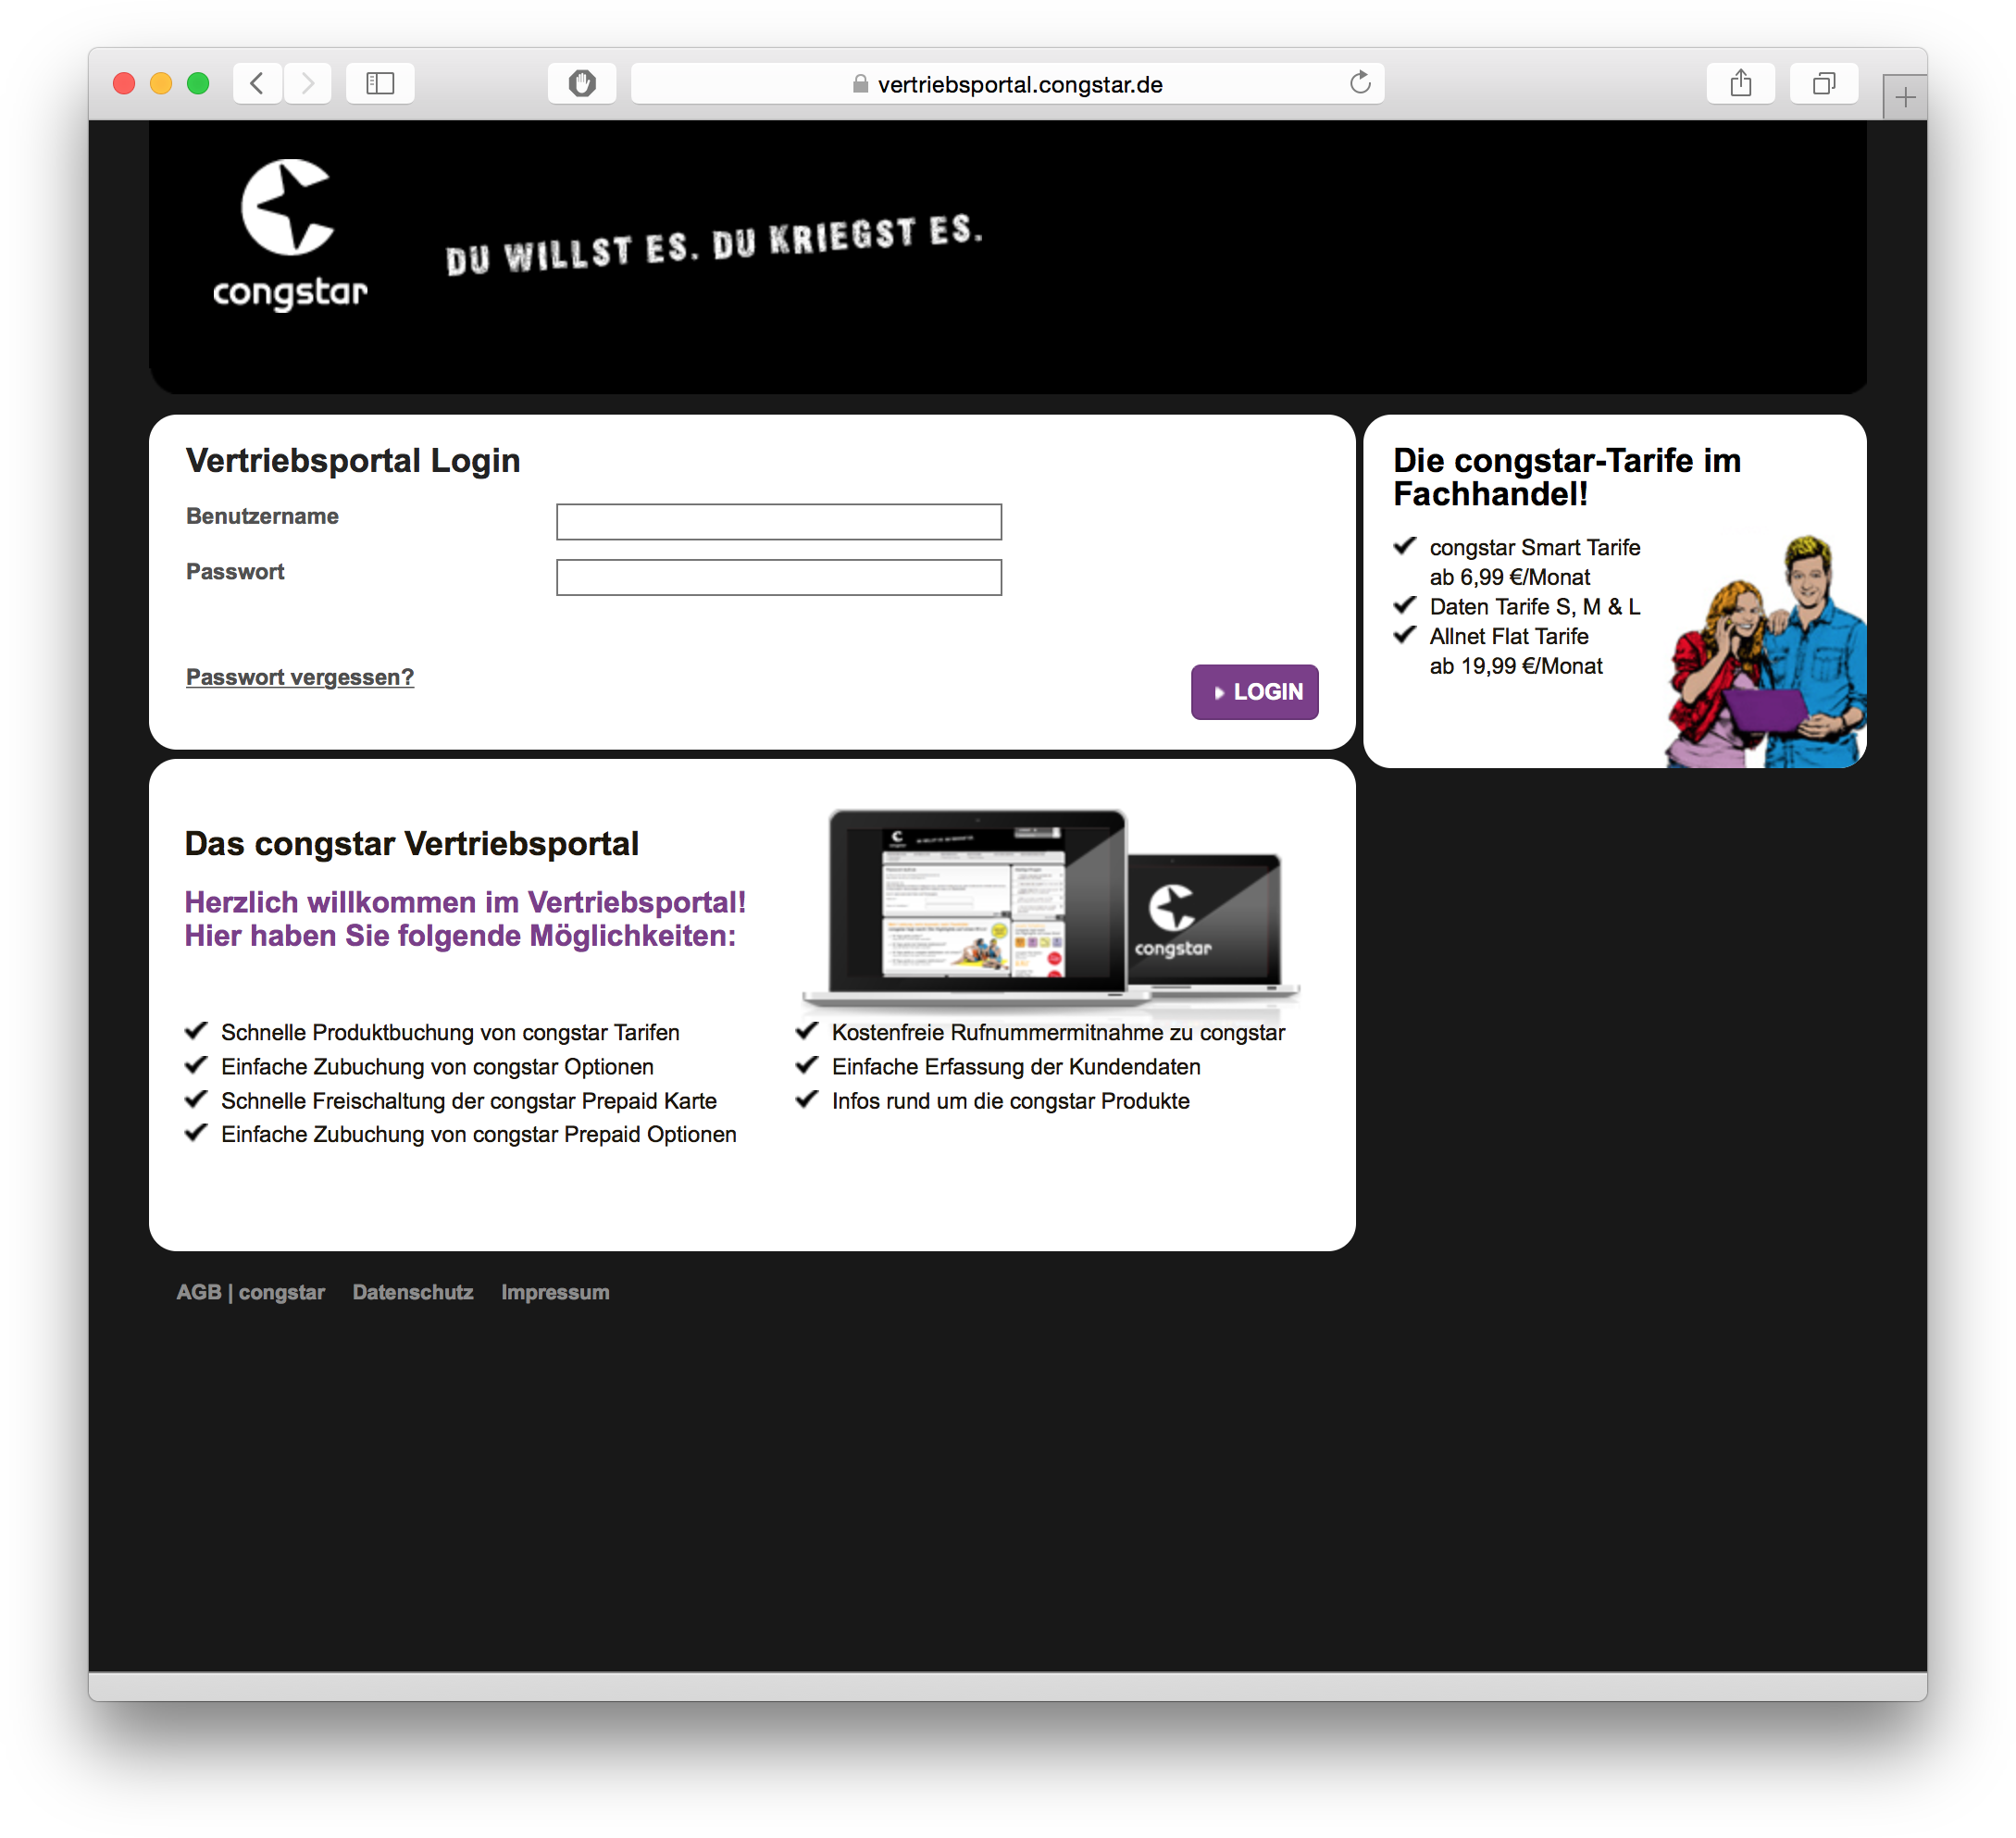
\includegraphics[width=0.7\textwidth]{images/Sites/Congstar_CPP.png}
\centering
\caption{Das Congstar Vertriebsportal (CPP) \cite{ccpp}}
\end{figure}

\pagebreak
Congstar Breitband:

\begin{figure}[H]
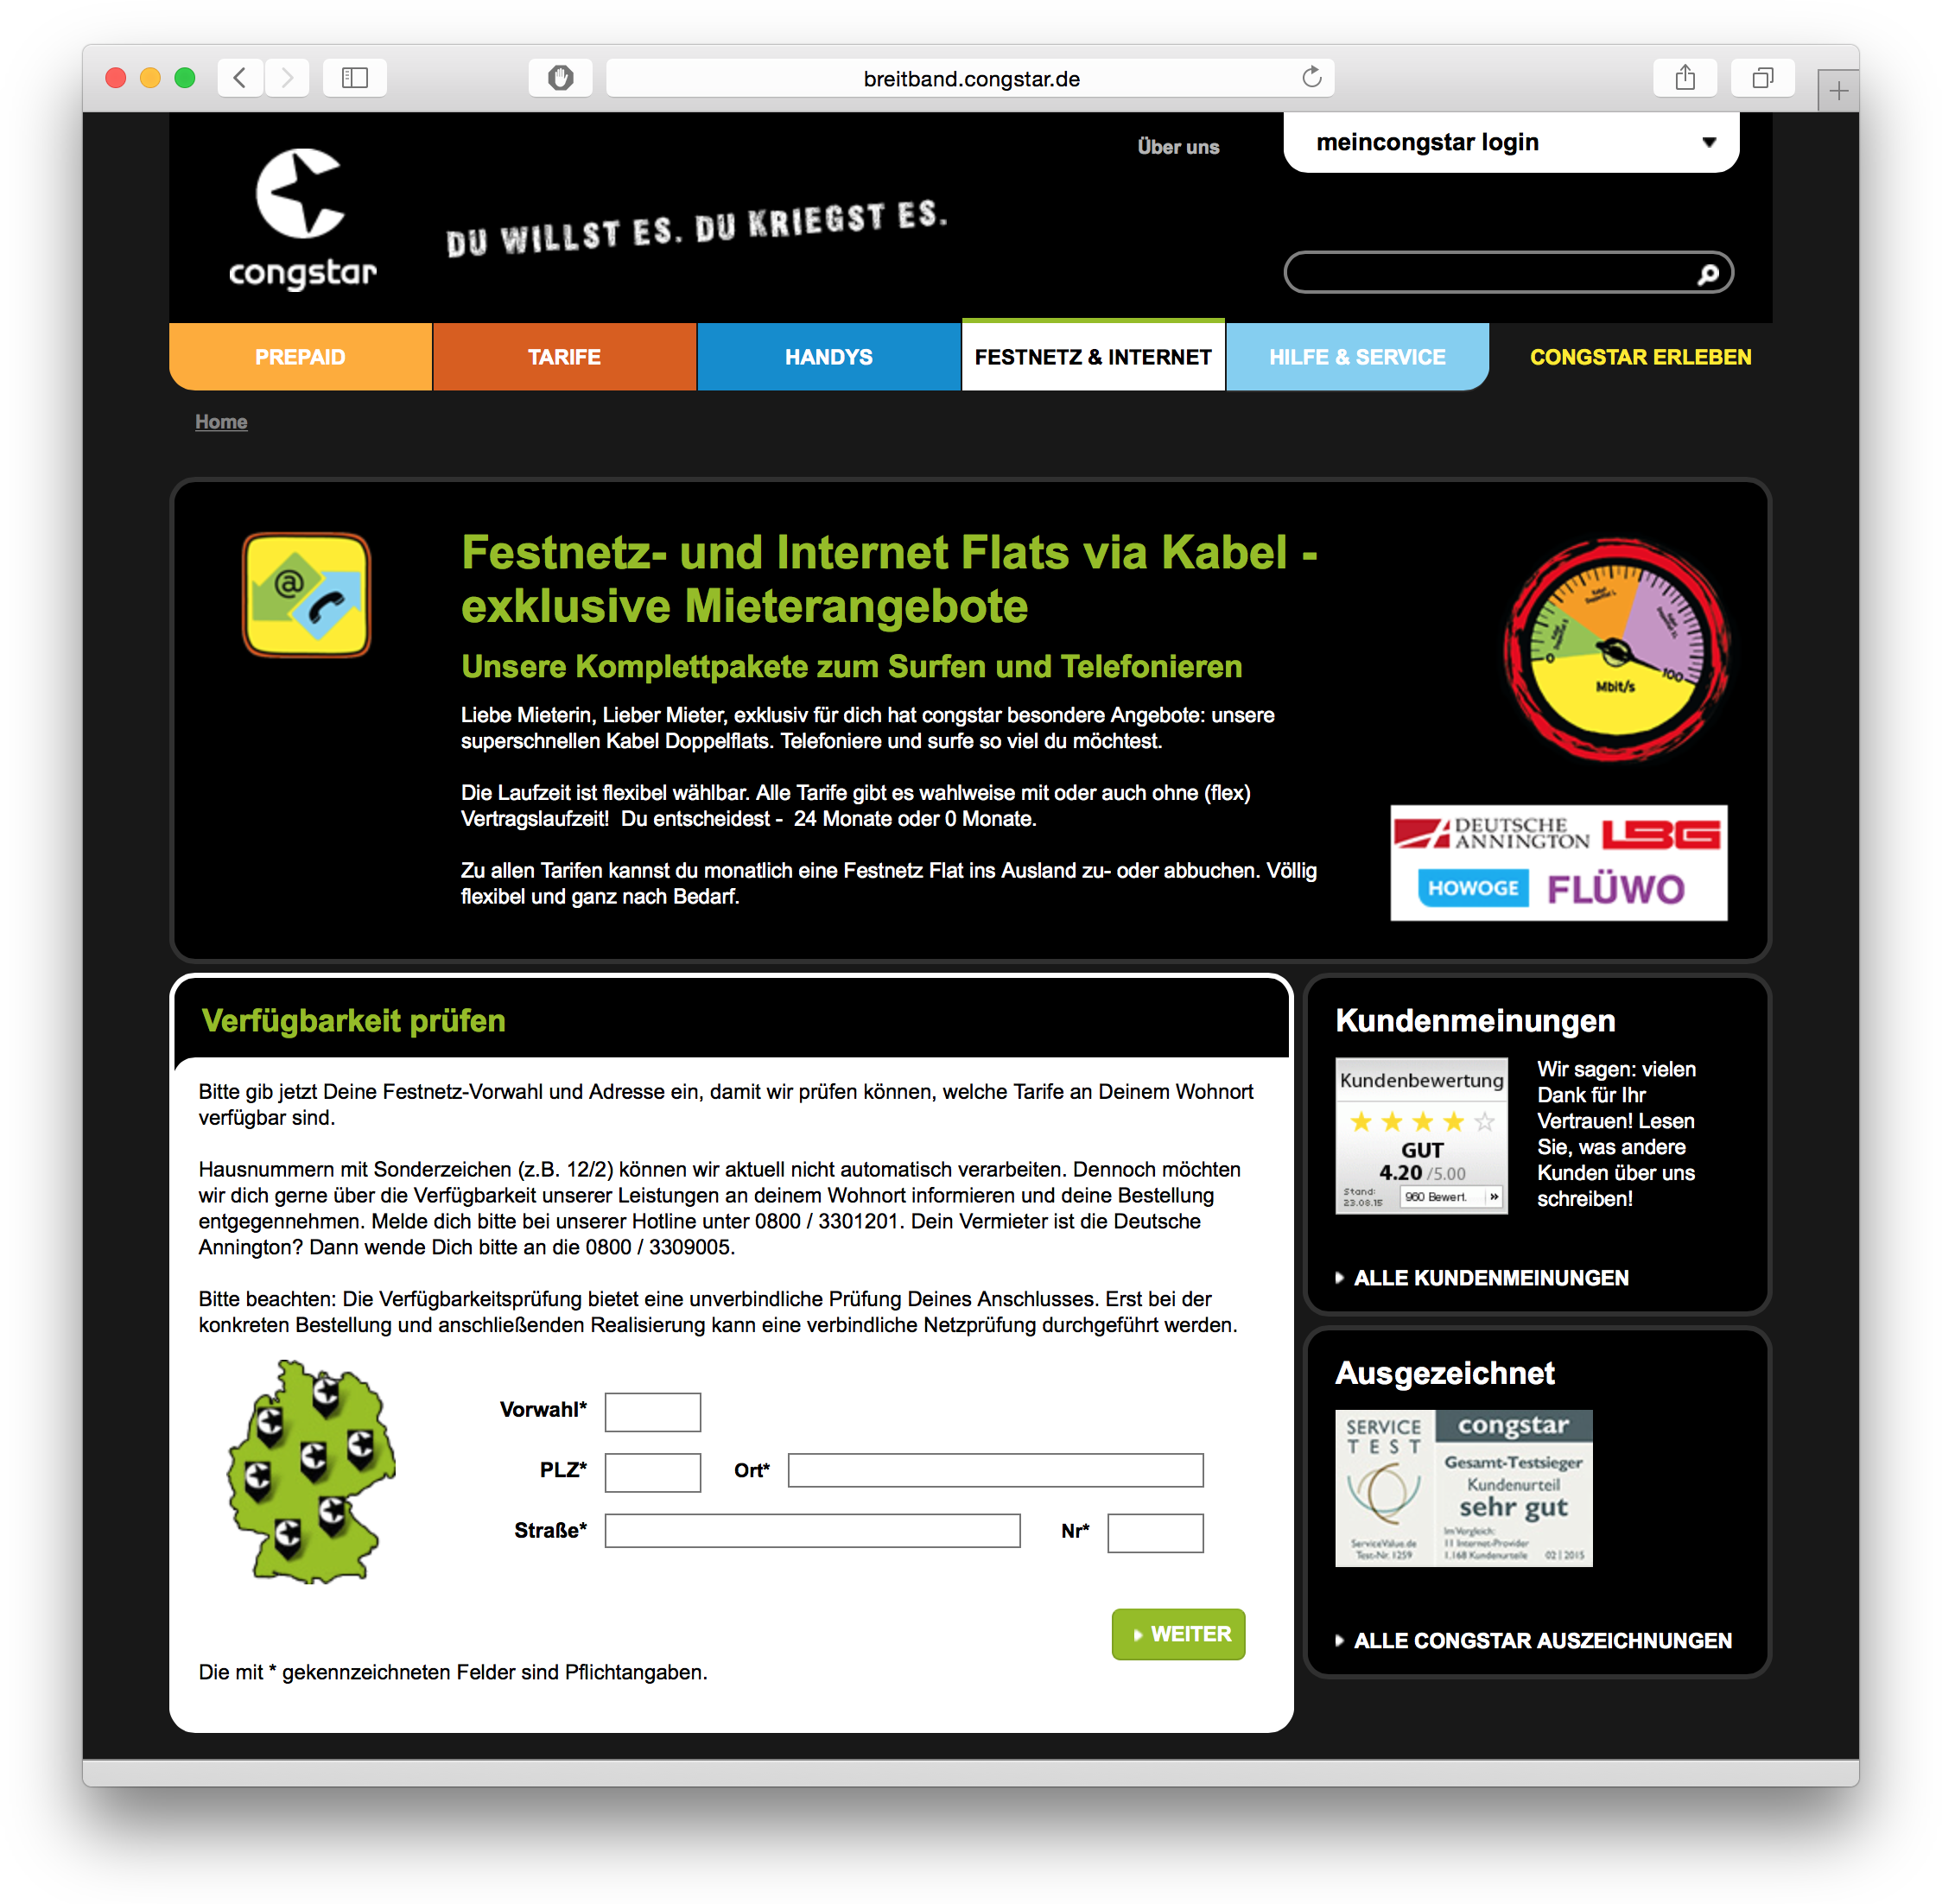
\includegraphics[width=0.7\textwidth]{images/Sites/Congstar_Breitband.png}
\centering
\caption{Die Congstar Breitband Hauptseite \cite{cb}}
\label{figure1}
\end{figure}

\begin{figure}[H]
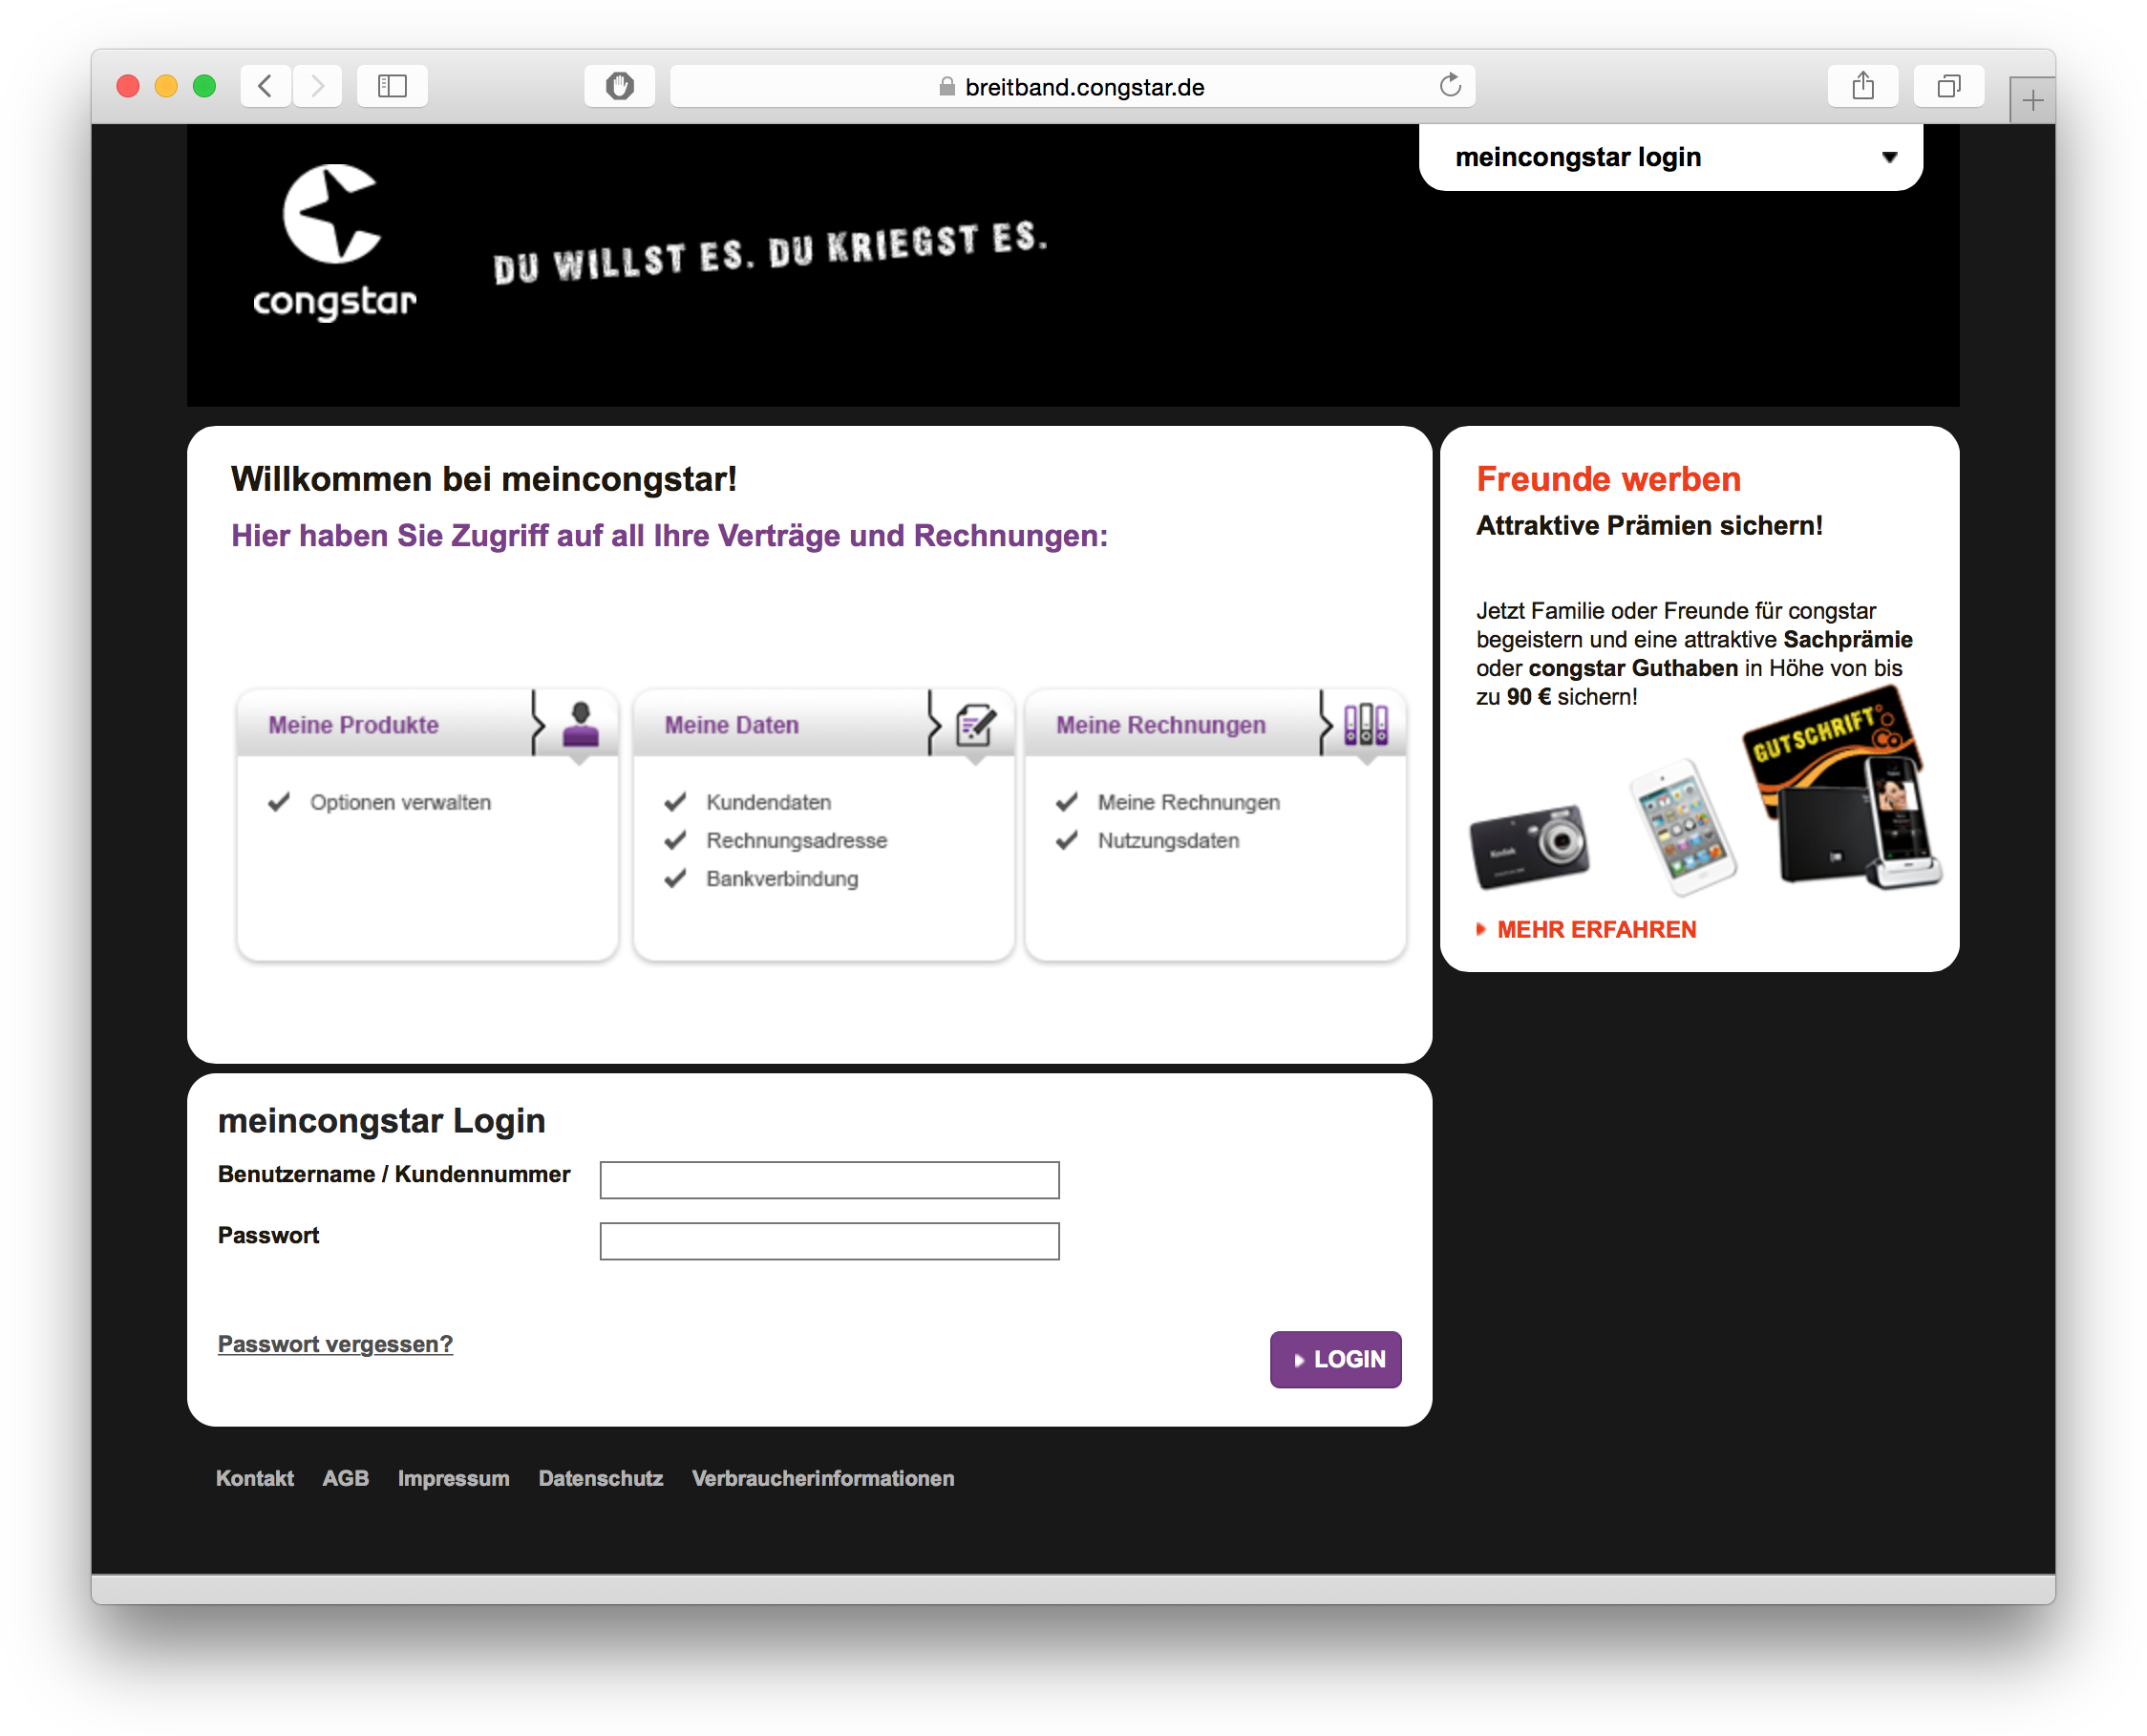
\includegraphics[width=0.7\textwidth]{images/Sites/Congstar_Breitband_CSC.png}
\centering
\caption{Das Congstar Breitband Kundenportal (CSC) \cite{cbcsc}}
\end{figure}

\pagebreak
White Label-Vertrieb:


\begin{figure}[H]

\includegraphics[width=0.7\textwidth]{images/Sites/White_Label/Ja_Mobil.png}
\centering
\caption{White Label - Die Ja! Mobil Webseite \cite{ja}}
\end{figure}

\begin{figure}[H]
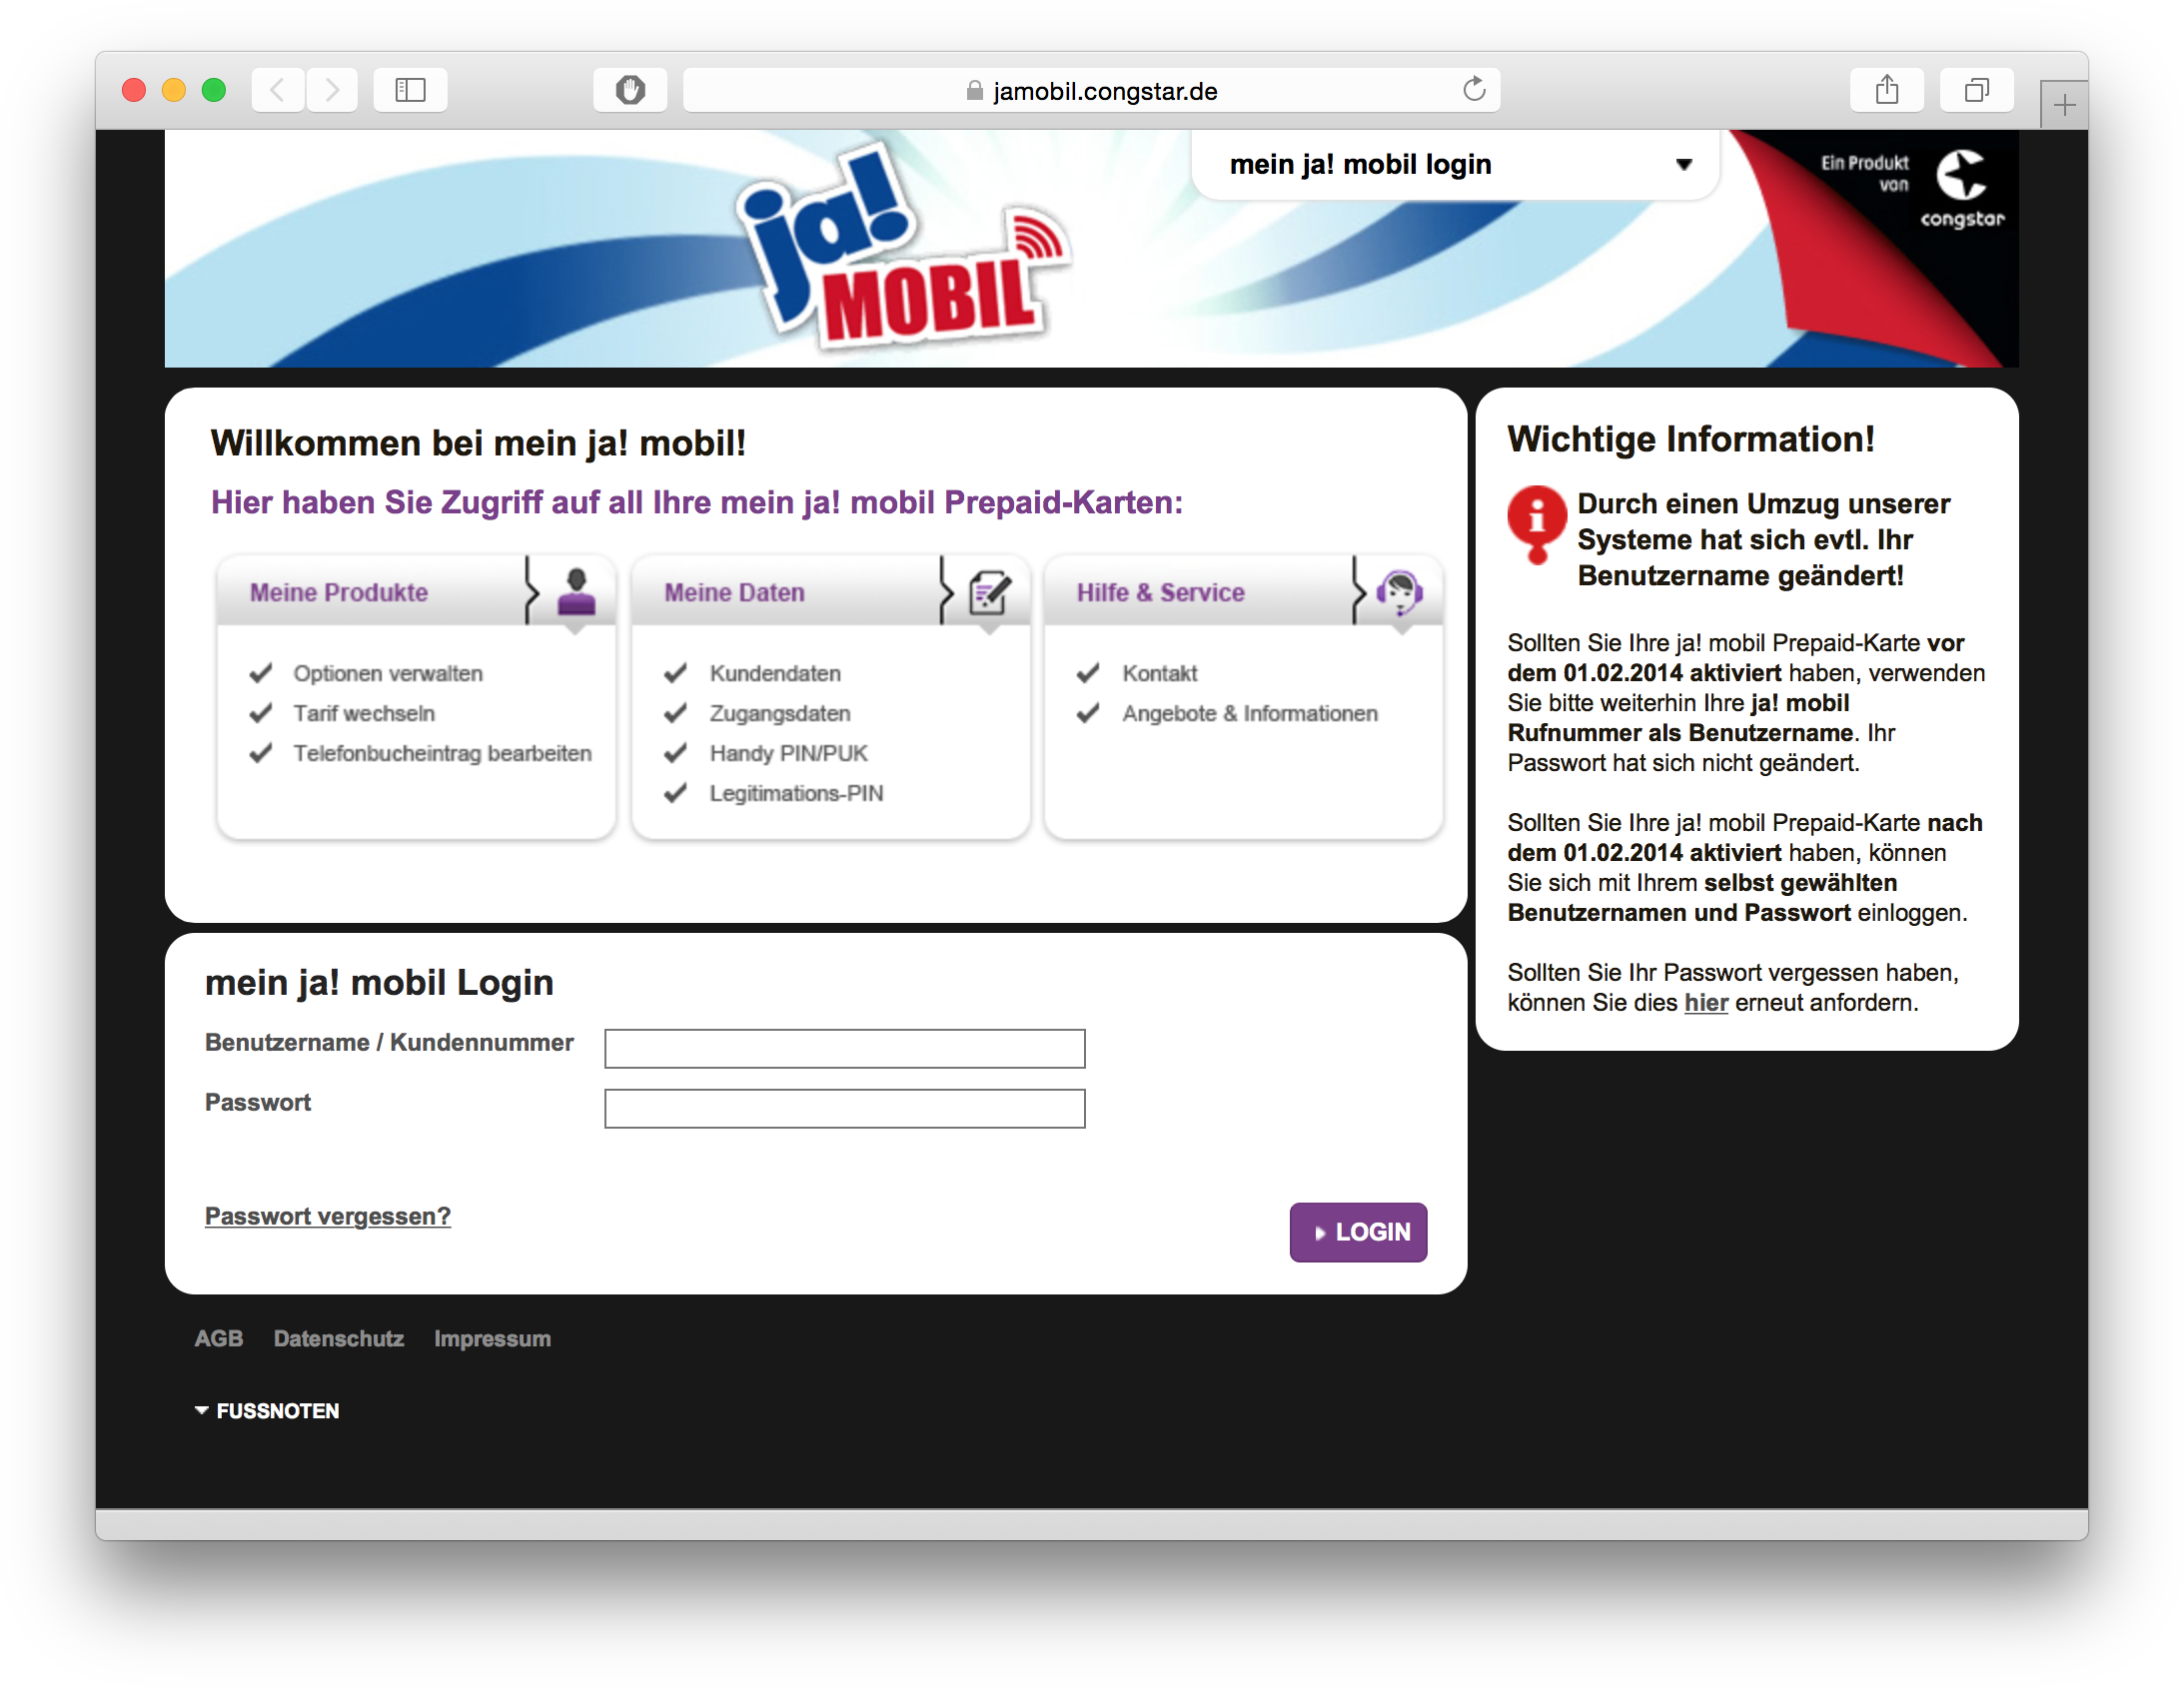
\includegraphics[width=0.7\textwidth]{images/Sites/White_Label/Ja_Mobil_CSC.png}
\centering
\caption{White Label - Das Ja! Mobil Kundenportal (CSC) \cite{jacsc}}
\end{figure}


\begin{figure}[H]
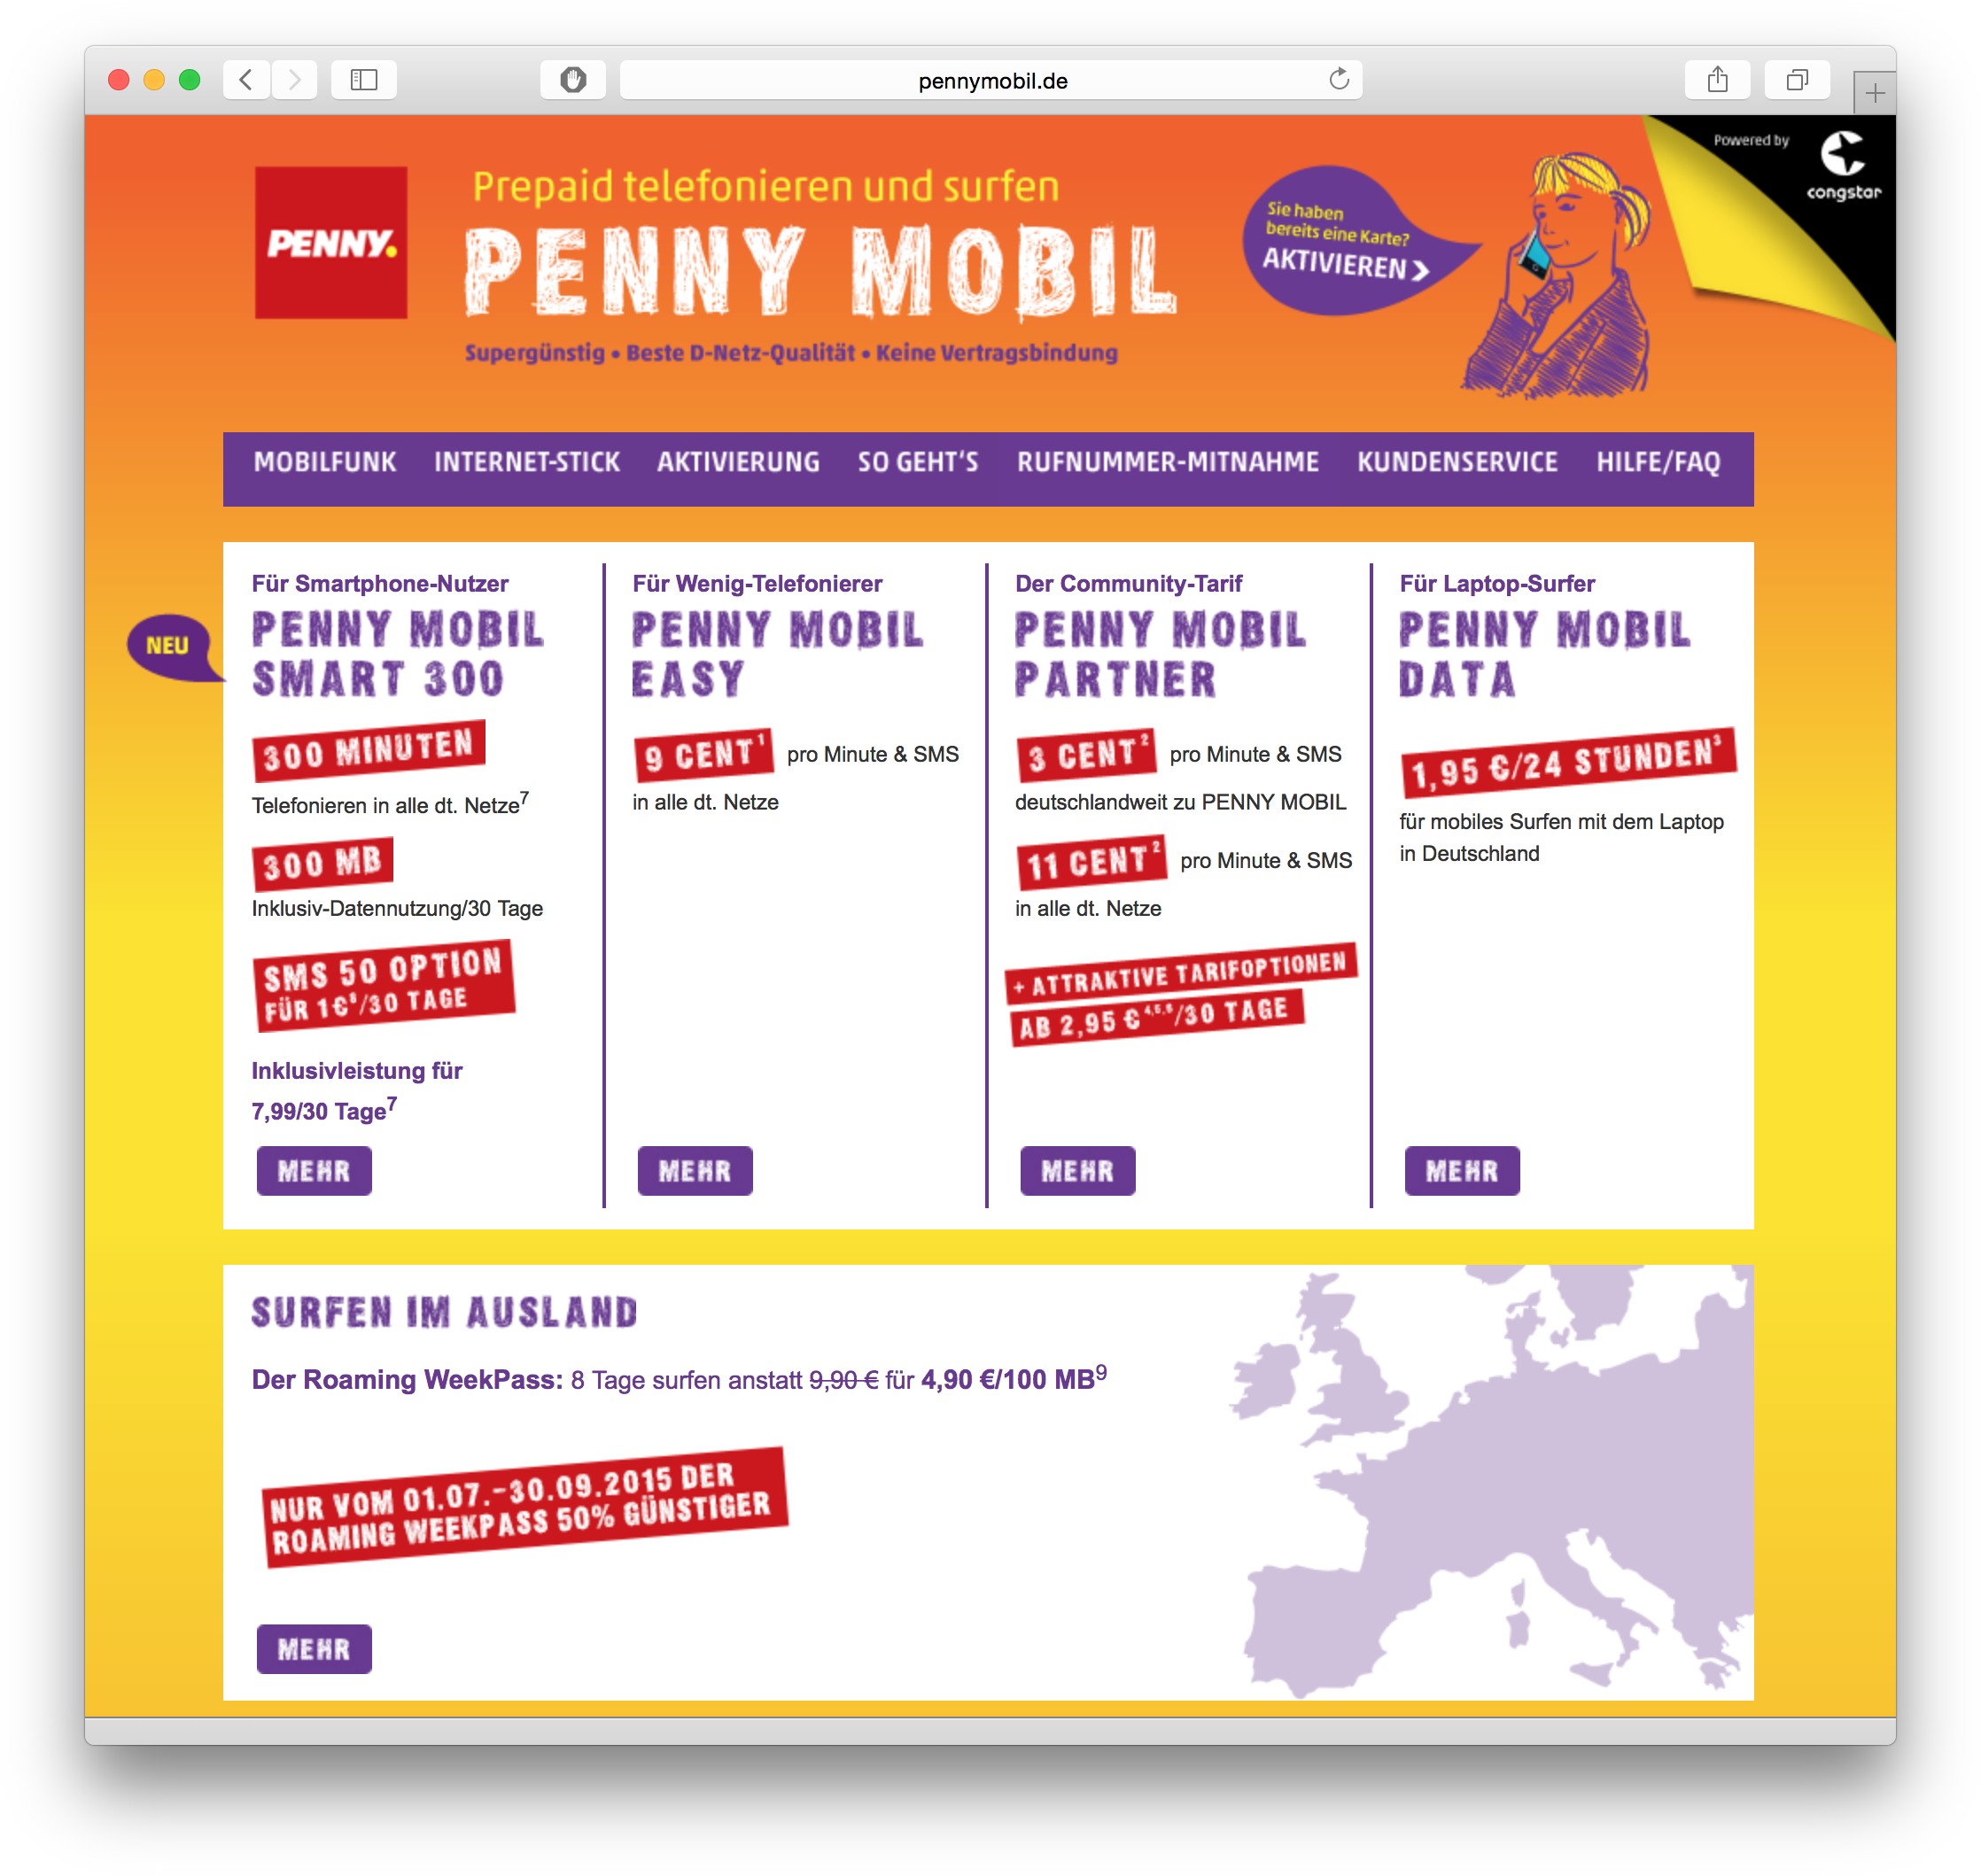
\includegraphics[width=0.7\textwidth]{images/Sites/White_Label/Penny_Mobil.png}
\centering
\caption{White Label - Die Penny Mobil Webseite \cite{penny}}
\end{figure}

\begin{figure}[H]
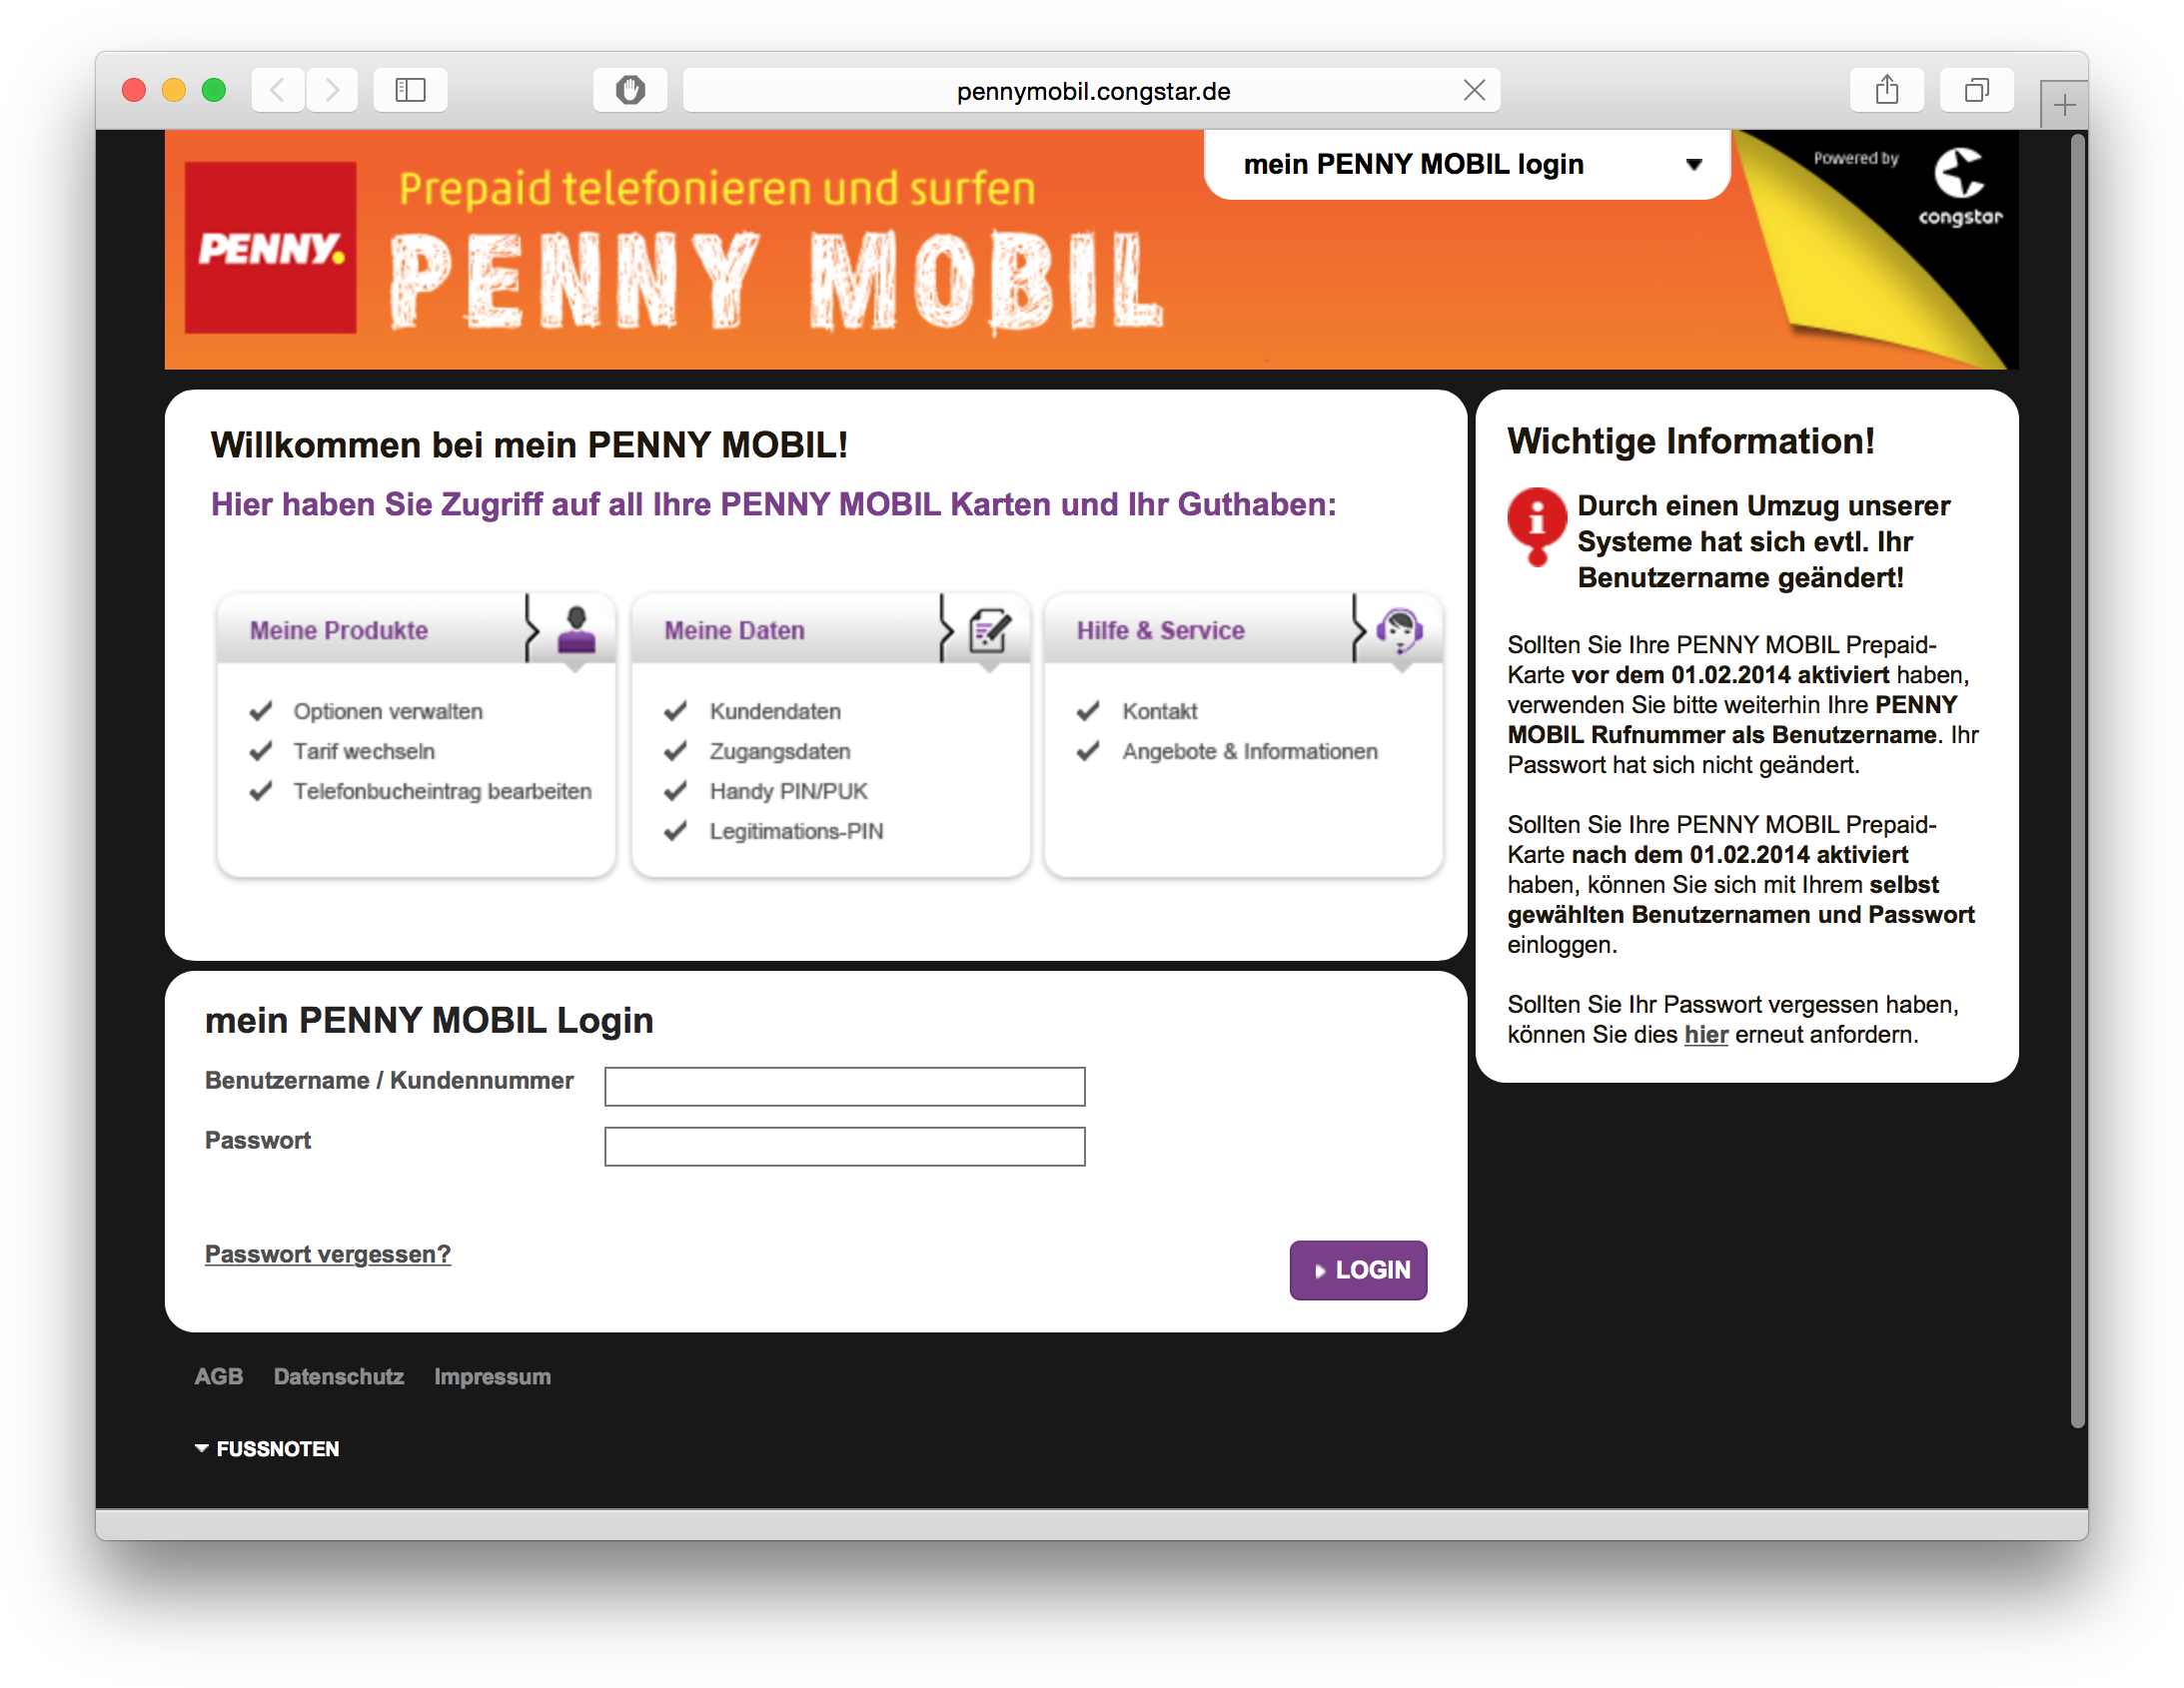
\includegraphics[width=0.7\textwidth]{images/Sites/White_Label/Penny_Mobil_CSC.png}
\centering
\caption{White Label - Das Penny Mobil Kundenportal (CSC) \cite{pencsc}}
\end{figure}

\pagebreak

\subsection{Umsetzung}

Die Web-Plattform ist in eine Gesamtarchitektur eingebettet, zu der auch ein zentrales Bestellmanagement- und Workflowsystem sowie ein Billingsystem gehört. Für das Thema Workflow ist die österreichische Firma Compax zuständig, um die Billing-Abwicklung kümmerte sich die Firma mr. nexnet.

Eines der Hauptziele war und ist die redundanzfreie Datenpflege und – auf die agilen Geschäftsanforderungen zugeschnittene – Konfigurationsmöglichkeiten. Dies wurde durch vielfälltige Konfigurationsmöglichkeiten in TYPO3 umgesetzt.

So können congstar-Kampagnen und Landing Pages von Marketing- und Sales-Mitarbeitern selbst direkt aus der Plattform heraus erstellt und verwaltet werden. Da durch gewinnt congstar sehr viel Zeit: Vorher dauerte es rund sechs Monate, bis ein Produkt auf dem Markt war. Heute konnte die so genannte “Time-to-Market“ auf wenige Tage verkürzt werden. In nur fünf Minuten ist eine neue Kampagne konfiguriert und online gestellt.

Ein weiteres Hauptziel des Projekts des Online-Vertriebs ist die Content-Personalisierung. TYPO3 ermöglicht Redakteuren, Content zielgruppenspezifisch anzulegen: So verändern sich z.B. Preise oder Angebote, je nach Einsprung-Link, über welchen die User auf die jeweilige Seite gekommen sind. Selbst auf das individuelle Benutzer-Verhalten, ob Bestandskunde oder Interessent, reagiert das System entsprechend.

Ein weiterer Fokus liegt auf dem Kundenservice: Die Vertragsstrukturen bei congstar sind flexibel und können vom Kunden modular zusammengestellt und verändert werden. Dies muss ebenfalls online geschehen und somit Kosten für congstar reduzieren. Über das CMS lässt sich das so genannte Customer Self Care (CSC) schnell und einfach durch Redakteure anpassen und pflegen.

Die gesamte Lösung “E-Commerce-Framework for Telcos“ oder kurz “EFT“ wurde von AOE speziell für den Einsatz im Bereich Telekommunikation entwickelt und bei congstar implementiert.

Heute wird das Gesamtsystem von ca. fünf Millionen Besucher am Tag und Tausend Bestandskunden besucht und genutzt.




\section{Deployment Pipeline} \label{sec:pipeline}

Im folgenden wird der Ablauf der Deployment-Pipeline erläutert.

\begin{figure}[H]
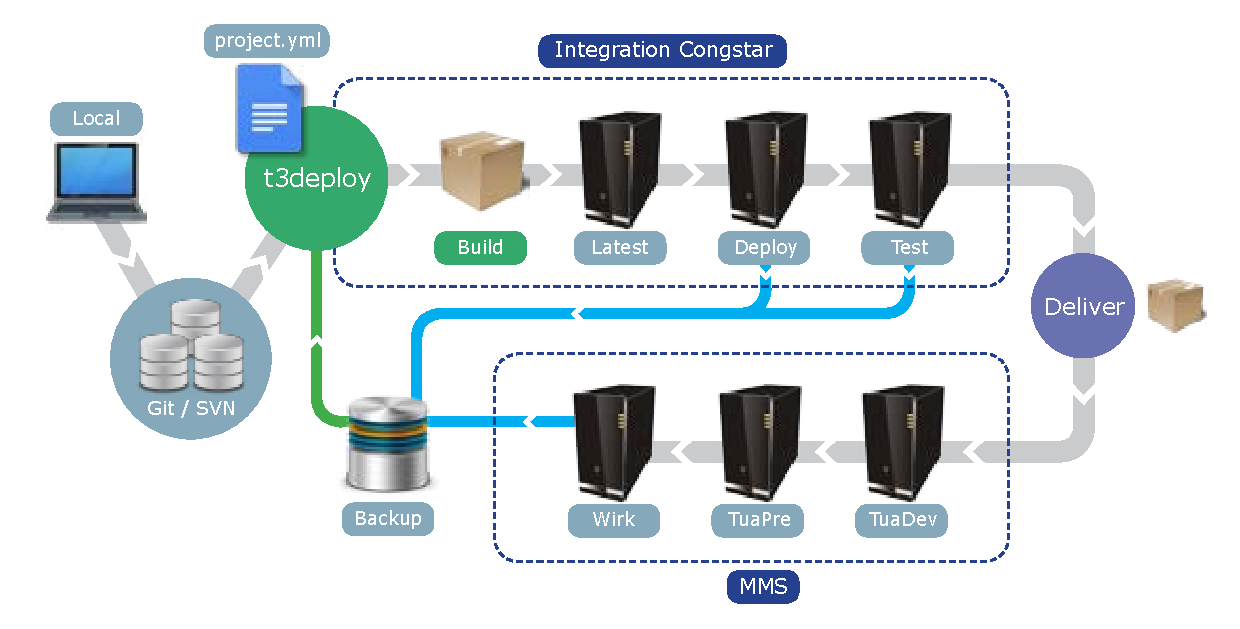
\includegraphics[width=\textwidth]{images/DeploymentPipeline.pdf}
\caption{Der Ablauf der Congstar Deployment-Pipeline }
\centering
\end{figure}

Der grobe Ablauf des Deployments sieht so aus, dass ein aktuelles Backup aller System, auf denen relevante Daten gepflegt werden müssen, erstellt und in den Backupstorage geschrieben wird. Dabei werden die Systeme vor einem Deployment gesperrt um zu verhindern, dass die Daten nach dem Backup noch verändert werden.

Die verschiedenen Systeme unterteilen sich in zwei Hauptkomponenten:
\begin{itemize}
  \item Integration Congstar
  \begin{itemize}
    \item wird von AOE gehostet
    \item beinhaltet die internen Deploy-Systeme (VM Ware Server)
    \item Voller Zugriff / volle Verantwortung bei AOE
    \item AOE Teil der Deployment Pipeline
  \end{itemize}
  \item MMS (T-Systems Multimedia Solution)
  \begin{itemize}
    \item wird von der Telekom Tochter MMS gehostet
    \item beinhaltet die externen Deploy-Systeme
    \item (Server Cluster mit verschiedenen Virtuellen Servern)
    \item Kein Einfluss / Zugriff durch AOE
    \item Congstar / MMS Teil der Deployment Pipeline
  \end{itemize}
\end{itemize}

Wird ein Softwarepaket komplett neu gebaut, wird zum einen der Quellcode aus den getagten Git-Repositories gezogen und zum anderen die Datenbank und andere Bewegungsdateien aus dem Backupstorage (jeweils von den relevanten Systemen) zusammengeführt.

Die Verheiratung findet mit der Deploymentsoftware T3Deploy statt. Mit Hilfe der Konfigurationsdatei project.yml baut die T3Deploy Software ein fertiges, installierbares Softwarepaket. Die Konfigurationsdatei enthält dabei alle Infomationen über Extensions, Libraries und Datenbanken, die zum Bau eines Pakets notwendig sind.

War der Bau eines Pakets erfolgreich, wird dieses zur erst auf den AOE-internen Umgebungen des Integration Congstar installiert und durchläuft mehrere Teststufen.

Auf der Latest Umgebung werden alle automatisierten Tests durchgeführt. Dazu gehören Unit-Tests, Smoke Tests, sämtliche Code Metriken und Static Cache Tests. Laufen dort alle Tests durch kann das Paket auf der Deploy Umgebung installiert werden. Dort haben die Redakteure von Congstar die Möglichkeit redaktionelle Änderungen vorzunehmen. Zusätzlich werden auf dieser Umgebung neue Nutzer für das Typo3-Backend angelegt, die über das Backupstorage in jedem gebauten Paket zugänglich gemacht werden. Die letzte Umgebung des Integration Congstar bildet die Test Umgebung. Dort laufen hauptsächlich die Java Selenium Tests. Dies sind Tests bei welchen die Seite automatisiert aufgerufen wird und “durchgeklickt“ wird und somit geprüft ob alle Workflows klickbar sind und funktionieren.

Sind alle drei AOE-internen Teststufen durchlaufen wird einmal täglich nachts ein fertiges Paket an die MMS geliefert und dort auf der TuADev (Test und Abnahme) Umgebung installiert. Auf der TuADev Umgebung werden Abnahmetests seitens der Congstar Testern durchgeführt, die ebenfalls hauptsächlich Selenium Tests umfassen. Die TuADev Umgebung Umgebung ist außerdem ein Content Master. Das heißt, dass die Congstar Redakteure auf diesem System neuen Content einpflegen können, wie zum Beispielsweise Seiten für neue Features anlegen oder den Inhalt der Seiten anpassen. Diese Option ist nötig, da die neuen Features zu dem Zeitpunkt noch nicht auf der Wirk Umgebung (Live System) enthalten sind und somit nur hier angepasst werden können. Ziel der Funktion ist es, dass beim Release direkt eine neue Funktion mit dem passenden redaktionell gepflegen Inhalt online geht.

Zu jedem Release wird zuerst die TuAPre Umgebung deployed, da diese dem Wirk System hinsichtlich der Konfiguration am nähesten ist.
Dies wir am Tag des Release durchgeführt um erste Probleme oder Fehler auszuschließen.

Das Wirk Deployment wird über Nacht durchgeführt um möglich wenig den laufenden Betrieb zu stören. Im Wirksystem gibt es sechs Webserver, welche hinter einer Lastverteilung arbeiten. Auf der Wirk Umgebung wird ein A/B Deployment durchgeführt, also die hälfte der Webserver wird offline genommen und installiert, sobald diese fertig sind, gehen diese wieder online und die andere hälfte wird offline genommen zum Deployment. Sobald diese dann auch die neue Software enthalten gehen sie wieder online.
Durch diese Technik ist jederzeit eine Erreichbarkeit der WebApplikation gesichert.




\section{Task 01: Extension zur Reisekostenkalkulation} \label{sec:pipeline}

Da viele Softwaremodule des Congstar Webshop und Vertriebsportal also Typo3 Extension umgesetzt sind, habe ich im Zuge 
meiner Einarbeitung eine eigene Extension entwickelt, die als Reiseplanungstool eingesetzt werden kann.
Ziel der Extension ist es, Personen eine grobe Kalkulation der Kosten offenzulegen, über Reiseziele, 
die sie gerne bereisen würden, von denen sie aber nicht wissen, welche Kosten auf sie zukommen. 
Informationen über Reiseziele und mögliche Kosten sollen über entsprechende APIs angesprochen werden und wurden bei der Umsetzung dieser Extension vernachlässigt.
Der Schwerpunkt der Umsetzung lag in der Erstellung und Konfiguration der Extension, sodass Sie über das
Typo3 Backend eingebunden werden kann und mit zugewiesener URL im Browser aufrufbar ist.




\section{Task 02: Rollen-basierte Zuordnung der Bestandskundenverwaltung} \label{sec:t02}

Ziel war es, dass die Bestandskundenfunktionalität rollen-basiert zugeordnet werden kann, 
damit sie nur den Sales-Partnern zur Verfügung steht, die die Funktion auch nutzen dürfen.

Dafür wurde im Typo3 Backend eine neue Gruppe für die Bestandskunden-Buchung angelegt.
Redakteure können dadurch die Zuordnung der Rechte im Typo3 für verschiedene Partner freischalten
oder zusätzlich zuweisen.

Zusätzlich wurde die Funktionalität des Sales-Partner-Objektes erweitert, sodass dieser Auskunft geben kann, 
welche Gruppe er inne hat. Dadurch wird für den jeweiligen Sales-Partner im Congstar Vertriebsportal,
nur die Funktionalität zur Verfügung gestellt, die ihm zugeordnet ist.




\section{Task 03: Content Box erstellen und anzeigen}

Damit Kunden bei der POS Kartenaktivierung informiert werden, wie sie den Congstar Mixer bei der POS Kartenaktivierung
nutzen können, soll oberhalb vom Mixer eine Content Box eingeblendet werden, die eine Beschreibung beinhaltet.
Dafür wurde in der eft Extension eine neue Flexform angelegt für die Content Box angelegt.
Diese wurde so konfiguriert, dass die Content Box im Typo3 Backend von den Redakteuren redaktionell pflegbar ist.
Weiter galt es zu beachten, dass die Content Box zum einen nur angezeigt werden soll,
wenn es sich um ein 9ct. Prepaid Madeira Produkt handelt und zum anderen nur wenn der Mixer angezeigt wird.
Dazu wurde sowohl die Logik im Controller angepasst, als auch das bestehende Template erweitert.




\section{Task 04: Webservice für den Kundenservice implementieren}

Aufgabe war es, die API der eft Extension um die Kunden-Authentifizierung zu erweitern.
Die API der eft Extension ruft dabei über einen Webservice die AAX$^2$ auf, um den Kunden zu authentifizieren.
Dies geschieht über einen SOAP call 
\begin{lstlisting}
public function authenticateByMtan($customerId, $mTan)
\end{lstlisting}
bei der eine mTan und die Kundennummer an die AAX$^2$ übergeben wird.
War die Kundenauthentifizierung erfolgreich, so liefert die AAX$^2$ ein Kunden-Objekt zurück, welches
danach in der Session gespeichert wird.
Treten jedoch Fehler auf, sollen folgende Exceptions diese abfangen:

\begin{itemize}
	\item EFT-API wirft Exception A, wenn mTan falsch/ungültig
	\item EFT-API wirft Exception B, wenn mTan abgelaufen (das passiert nach 20 Minuten)
	\item EFT-API wirft Exception C, wenn der Webservice der AAX$^2$ nicht verfügbar ist
\end{itemize}




\section{Task 05: Konfiguration eines Jenkins Job}

\subsection{Schritt 1: build.xml mit Ant ohne Jenkins erstellen}
Zunächst einmal war es Ziel zu verstehen, wie eine build.xml aufgebaut ist
und aus welchen Befehlen sie besteht, um im Nachgang nachvollziehen zu können, auf welchen
Grundlagen die Einstellungen im Jenkins aufbauen.

$TODO$ einfach eine build.xml einer Extension öffnen und die wichtigsten Schritte beschreiben

\subsection{Schritt 2: Build-Job mit Jenkins konfigurieren}

$TODO$ Einrichtung eines Build-Jobs der für den Bau und das Testen
der Extension $congstar_eft_rest_api$ zuständig ist.
- Dabei muss konfiguriert werden unter welchen Repository, die Extension zu finden ist.
- PHPMD




\section{Task 06: Erstellung von Databuildern}

$TODO$ Im Zuge dieses Tasks wurden DataBuilder erzeugt, die das Generieren von Mock-Objekten in Unit-Tests erleichtert.

$TODO$ Beispiel-Code 
$TODO$ Erläuterung wieso DataBuilder in dem Fall sinnvoll sind




\section{Task 07: Durchstich OptionsGroups}

$TODO$ Beschreibung als $eft_core$ extrahieren




\section{Task 08: Durchstich ContractDuration}

$TODO$ Beschreibung aus $eft_core$ extrahieren
CR 5539 - Madeira - Implementierung REST Endpoint "getOptions" (BE) (13P)
Description


Als Entwickler möchte ich den REST Endpoint "getOptions" implementieren.

Akzeptanzkriterien:

Controller in der neuen Extension
Abstimmung Datenstruktur (auch mit Hinblick auf Optionswechsel)
Optionsanreicherungen sind erweitert
"Schwestern-Option" (Referenz auf andere Option)
"ist-Turbo-Option" (Flag)
Hochreichen der Optionen in ein für das Frontend fertiges Format zur Darstellung
Folgende Elemente des Mixers sollen redaktionell pflegbar sein (siehe sto191):
Texte in "mehr Details" Layer
NEU: Beschreibung zum Datenturbo inkl. Preis-Info (ausgewählt und nicht ausgewählt)
"Mein Mix"-Beschreibung zum Datenschieber auf "0"
"Mein Mix"-Beschreibungen zu Telefonie und SMS auf "0"
Abstimmung mit AAX (Null-Option!?) (PO)
API Dokumentation erstellt
Profiling erstellt




\section{Task 09: Property hasMixableOptions an Produkt ergänzen}

$TODO$ nachschauen ob Konversion bei diesem Task mit inbegriffen war




\section{Task 10: Implementierung von CodeSniffern zur Überprüfung von Namespace-Deklaration, File Doc Comment und Use-Statements von PHP Dateien}

Die Aufgabe dieses Tasks, war die Implementierung von CodeSniffern zur Überprüfung
der eigens definierten Code-Style Richtlinien des Congstar Web-Teams. Die verschiedenen CodeSniffer 
überprüfen dabei, die Existenz und Reihenfolge von: Namespace-Deklaration, 
File Doc Comment und Use-Statements in PHP-Dateien. Wie im Code Block unten zu sehen, sollen 
folgende Richtlinien überprüft werden:

\begin{enumerate}
  \item Namespace-Deklaration ist vorhanden
  \item Namespace-Deklaration befindet sich direkt unterhalb des PHP-Opening-Tags \label{item1}
  \item nach der Namespace-Deklaration folgt eine Leerzeile \label{item2}
  \item nach \ref{item1}. und \ref{item2}. folgt das File Doc Comment
  \item das File Doc Comment beinhaltet die von Aoe vorgegebene Copyright Notice \label{item4}
  \item nach dem File Doc Comment folgt eine Leerzeile \label{item5}
  \item nach \ref{item4}. und \ref{item5} können Use-Statements folgen
  \item wenn Use-Statements vorhanden sind, müssen diese unterhalb des File Doc Comment stehen
  \item nach dem File Doc Comment oder nach den optionalen Use-Statements muss ein Leerzeile folgen
\end{enumerate}

\begin{lstlisting} 
<?php
namespace Aoe\Checkout\Domain\Model;
 
/***************************************************************
 *  Copyright notice
 *
 *  (c) 2015 AOE GmbH <dev@aoe.com>
 *
 *  All rights reserved
 ***************************************************************/
 
use Aoe\Checkout\Domain\Model\Customer\Address;
use Aoe\Checkout\Domain\Model\Customer\LoginData;
use Aoe\Checkout\Domain\Model\Customer\PersonalData;
use Aoe\Checkout\Domain\Model\Payment;
 
class Customer
...
\end{lstlisting} \label{codesniffer}

Die Umsetzung der CodeSniffer beruht auf Grundlage des PHP CodeSniffer Scripts von Squizlab 
\cite{SquizlabPHPCodeSniffer}. Dieses Script scannt zum Beispiel eine PHP-Datei und liefert
eine Liste aus Tokens, die den jeweiligen Inhalt der Datei beschreibt. Jedes Token beschreibt dabei,
beispielsweise einen PHP-Tag, Leerzeichen, Strings und vieles mehr. Aufbauend darauf
wurden die CodeSniffer implementiert. Jeweils für die Namespace-Deklaration, File Doc Comment
und Use-Statements wurde ein eigener CodeSniffer in Form einer PHP-Klasse implementiert.
Jede CodeSniffer-Klasse implementiert dabei das PHP CodeSniffer Sniff Interface, dass vorschreibt
die Methoden register() und process() zu implementieren. Die register Methode wird dazu 
verwendet zu definieren, auf welchen Tokens der Sniff losgelassen werden soll.
Die process Methode wird anschließend jedes mal aufgerufen, wenn das Script auf einen registrierten
Token stößt. Ausgehend von der process Methode wurde die eigentliche Logik und Überprüfungen
der Code-Style Richtlinien implementiert. Falls ein Verstoß gegen die Richtlinien 
aufgetreten ist wird ein Fehler oder Warnung geschmissen.
Diese Information bei einem auftretenden Fehler oder einer Warnung, wird in eine Output-Datei
geschrieben.

Nach der Erstellung der CodeSniffer mussten diese noch ins Projekt integriert werden.
Für jeden Extension beziehungsweise Komponente, für die die CodeSniffer eingesetzt werden sollen,
wurde der jeweilige Build-Job erweitert. Dafür musste die Einstellung des Jenkins Job der jeweiligen 
Komponente erweitert werden. Bei den Einstellungen für die verschiedenen Code Checkstyle Analysen,
wurde das Ausführen des PHP CodeSniffer Scripts phpcs unter Angabe des Pfads zu den entsprechenden zu
prüfenden Dateien angegeben. Zusätzlich wurde die Einstellung getroffen, dass das Ergebnis der CodeSniffer
in die Ausgabedatei checkstyle.xml hinzuzufügen. Dadurch ist es möglich innerhalb des Jenkins Job
visualisiert zu bekommen, wo eine Warnung oder Fehler aufgetreten ist.



\section{Task 11: Implementierung eines CodeSniffers zu Überprüfung von Code Coverage Ignore Annotationen}

Umsetzung eines weiteren CodeSniffers der den PHP Code auf Code Coverage Ignore Annotations prüfen soll.
Mit Hilfe der Code Coverage Ignore Annotations ist gezielt möglich Codezeilen, Methoden oder gar ganze 
Klassen, von den PHP Metriken unbeachtet zu lassen, sodass die Code Coverage nicht sinkt, falls für
diesen Code keine Unit Tests existieren. 
Es kann auch durchaus manchmal der Fall sein, dass solche Annotations Sinn machen, wenn Code beispielsweise
nicht testbar ist. Es war eine Teamentscheidung zu sagen, dass die Code Coverage für Unit Tests transparent zu
halten und somit auf Code Coverage Ignore Annotations zu verzichten.

Folgende Codebeispiele zeigen die Annotations auf die geprüft werden soll.

\begin{lstlisting} 
/**
 * @codeCoverageIgnore
 */
\end{lstlisting} 

\begin{lstlisting} 
// @codeCoverageIgnoreStart
... hier steht ein bisschen Code
// "codeCoverageIgnoreEnd
\end{lstlisting} 

Sobald eine solche Annotation im Code entdeckt wurde, wird eine Warnung geworfen, die später bei den Ergebnissen des Build-Jobs angezeigt wird.

\begin{figure}[h]
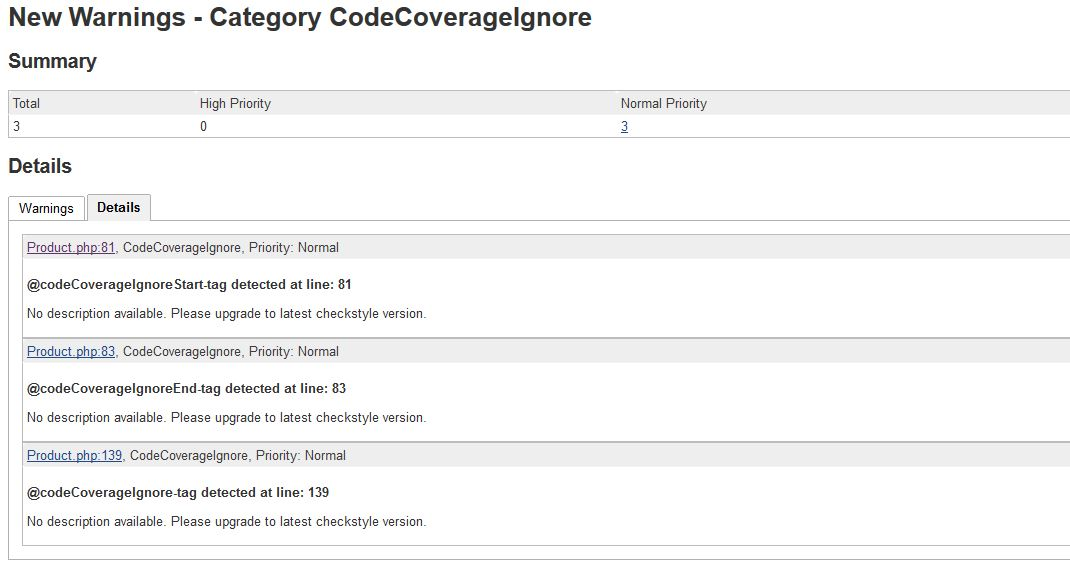
\includegraphics[width=\textwidth]{images/resultSniffer.JPG}
\centering
\end{figure}


\section{CodeReview}

Nachdem neuer Code entwickelt und durch Unit Tests getestet wurde, erstellt jeder Entwickler ein Code Review Task 
für den eigens geschriebenen Code. Dies geschieht im Congstar Team mit Hilfe von Crucible. Crucible ist ein Tool 
von Atlassien um Code Reviews zu erstellen. Den Code für das Code Review bezieht Crucible dabei direkt
aus den Git- und SVN-Repositories. Durch vorhanden sein der Repository Historie ist es möglich jeden Commit
mit ins Code Review aufzunehmen, um später gezielt Änderungen betrachten zu können. Der in Crucible sichtbare Code
kann dort direkt mit Kommentaren und Verbesserungsvorschlägen versehen werden.
Gegen Ende meines Praktikums vielen auch solche Task in meinen Aufgabenbereich.


\section{Behobene Issues} \label{sec:issues}

\subsection{Issue 01: Optionsmanagement CSC - Optimierung der Anzeige für gebuchte Optionen}

Congstar bieten seinen Kunden im CSC seines Webshops die Möglichkeit jederzeit neue Optionen dazu zu buchen oder umzubuchen.
Dabei gibt es Optionen in drei Kategorien: Optionen für SMS, für mobiles Internet und für Telefonie.
Für ein Tarif Produkt kann für jede Kategorie jedoch nur eine Option ausgewählt werden.

Thema dieses Issues war, dass auch bei drei gebuchten Optionen aus jeder Kategorie noch der Bereich anzeigt wird,
indem die zu buchbaren Optionen stehen sollten. 

Was fehlte war lediglich eine Überprüfung ob in jeder Kategorie bereits eine Option ausgewählt ist um das Template,
in einem solchen Fall ohne die zu-buchbaren Optionen anzuzeigen.

\begin{figure}[h]
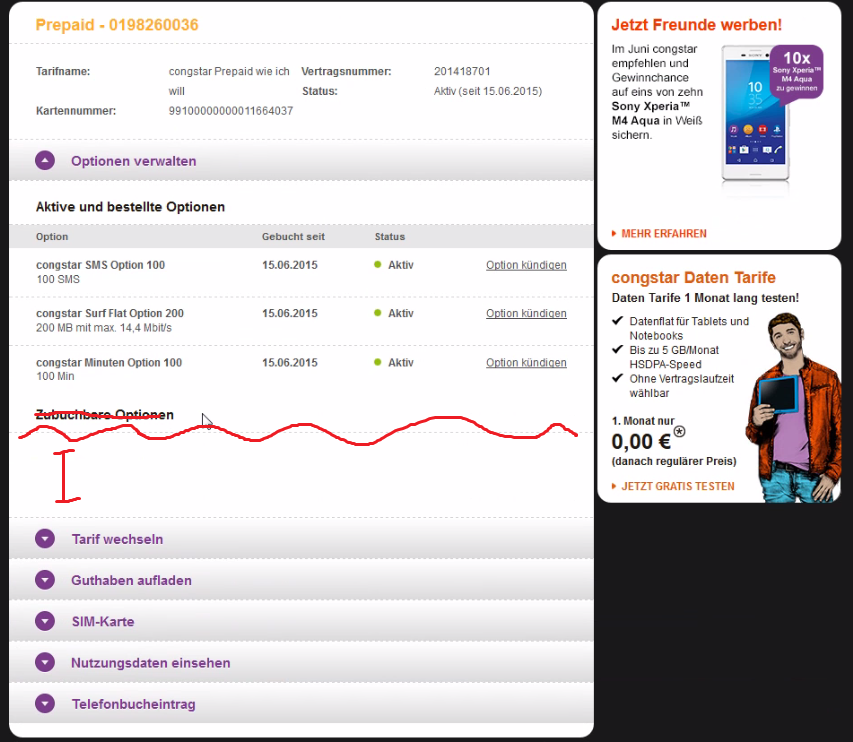
\includegraphics[width=\textwidth]{images/optionenzubuchung.PNG}
\centering
\end{figure}


\subsection{Issue 02: Abstände auf der MeineProdukte-Seite im CSC auf den Inhalt anpassen} \label{sec:issue02}

Das Problem bei diesem Issue bestand darin, dass der Style des Templates an einer bestimmten Stelle, für den Text
der Tarifnamen fest definiert war und so bei langen Tarifnamen, der Text unschön umgebrochen ist.
Hier mussten lediglich Änderungen im SCSS vorgenommen werden, wodurch ich den Umgang mit SASS und compass
kennengelernt habe.


\subsection{Issue 03: Abstände auf der MeineProdukte-Seite (Übersicht) im CSC auf den Inhalt anpassen} 

Ähnlich wie in Issue \ref{sec:issue02} waren hier Änderungen im SCSS für ein Template notwenig, sodass
der Tarifname bei der Produktübersichtsseite nicht mehr umbricht.


\subsection{Anpassung des Hinweistexts zur Triple-SIM} 

Nach Auswahl eines Tarifs und Auswahl eines Handys für diesen Tarif, gelangt im nächsten Schritt 
auf die Auswahlseite für die Simkarte. In der Vergangenheit bestand die Möglichkeit abhängig vom
Simkartentyp des Handys zwischen einer Nano, Hybrid oder Triple Simkarte zu wählen.

Inzwischen ist es jedoch so das unabhängig vom Gerät und benötigter Simkarte nur noch die Triple Simkarte
ausgeliefert wird. Diese bietet für alle Gerätetypen, die passende Simkarte bereit.

Wie in Abbildung \ref{fig:triple} treten bei der Anzeige der verschiedenen Informationen noch Fehler auf.

\begin{figure}[h] \label{fig:triple}
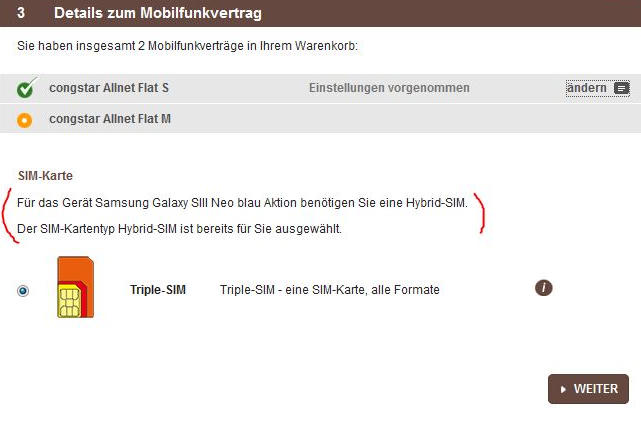
\includegraphics[width=\textwidth]{images/triple.PNG}
\caption{vorausgewählte Triple Simkarte \cite{ccpp}}
\centering
\end{figure}

$$TODO$$



\newpage

\bibliographystyle{plain}
\bibliography{online}


\end{document}
